\PassOptionsToPackage{unicode=true}{hyperref} % options for packages loaded elsewhere
\PassOptionsToPackage{hyphens}{url}
%
\documentclass[ignorenonframetext,]{beamer}
\setbeamertemplate{caption}[numbered]
\setbeamertemplate{caption label separator}{: }
\setbeamercolor{caption name}{fg=normal text.fg}
\beamertemplatenavigationsymbolsempty
\usepackage{lmodern}
\usepackage{amssymb,amsmath}
\usepackage{ifxetex,ifluatex}
\usepackage{fixltx2e} % provides \textsubscript
\ifnum 0\ifxetex 1\fi\ifluatex 1\fi=0 % if pdftex
  \usepackage[T1]{fontenc}
  \usepackage[utf8]{inputenc}
  \usepackage{textcomp} % provides euro and other symbols
\else % if luatex or xelatex
  \usepackage{unicode-math}
  \defaultfontfeatures{Ligatures=TeX,Scale=MatchLowercase}
\fi
\usetheme[]{metropolis}
\usecolortheme{seahorse}
\usefonttheme{structuresmallcapsserif}
% use upquote if available, for straight quotes in verbatim environments
\IfFileExists{upquote.sty}{\usepackage{upquote}}{}
% use microtype if available
\IfFileExists{microtype.sty}{%
\usepackage[]{microtype}
\UseMicrotypeSet[protrusion]{basicmath} % disable protrusion for tt fonts
}{}
\IfFileExists{parskip.sty}{%
\usepackage{parskip}
}{% else
\setlength{\parindent}{0pt}
\setlength{\parskip}{6pt plus 2pt minus 1pt}
}
\usepackage{hyperref}
\hypersetup{
            pdftitle={Advances on a computational tool for patient-specific dosimetry in nuclear medicine},
            pdfborder={0 0 0},
            breaklinks=true}
\urlstyle{same}  % don't use monospace font for urls
\newif\ifbibliography
\usepackage{graphicx,grffile}
\makeatletter
\def\maxwidth{\ifdim\Gin@nat@width>\linewidth\linewidth\else\Gin@nat@width\fi}
\def\maxheight{\ifdim\Gin@nat@height>\textheight\textheight\else\Gin@nat@height\fi}
\makeatother
% Scale images if necessary, so that they will not overflow the page
% margins by default, and it is still possible to overwrite the defaults
% using explicit options in \includegraphics[width, height, ...]{}
\setkeys{Gin}{width=\maxwidth,height=\maxheight,keepaspectratio}
% Prevent slide breaks in the middle of a paragraph:
\widowpenalties 1 10000
\raggedbottom
\setbeamertemplate{part page}{
\centering
\begin{beamercolorbox}[sep=16pt,center]{part title}
  \usebeamerfont{part title}\insertpart\par
\end{beamercolorbox}
}
\setbeamertemplate{section page}{
\centering
\begin{beamercolorbox}[sep=12pt,center]{part title}
  \usebeamerfont{section title}\insertsection\par
\end{beamercolorbox}
}
\setbeamertemplate{subsection page}{
\centering
\begin{beamercolorbox}[sep=8pt,center]{part title}
  \usebeamerfont{subsection title}\insertsubsection\par
\end{beamercolorbox}
}
\AtBeginPart{
  \frame{\partpage}
}
\AtBeginSection{
  \ifbibliography
  \else
    \frame{\sectionpage}
  \fi
}
\AtBeginSubsection{
  \frame{\subsectionpage}
}
\setlength{\emergencystretch}{3em}  % prevent overfull lines
\providecommand{\tightlist}{%
  \setlength{\itemsep}{0pt}\setlength{\parskip}{0pt}}
\setcounter{secnumdepth}{0}

% set default figure placement to htbp
\makeatletter
\def\fps@figure{htbp}
\makeatother


\title{Advances on a computational tool for patient-specific dosimetry in
nuclear medicine}
\author{\textbf{P. Pérez}\\
IFEG-CONICET \& FAMAF-UNC, Argentina\\
~\\
\textbf{\emph{VI Conferencia de Física Médica en la Frontera}}\\
November 7, 2018}
\date{\begin{center}
\vspace{1cm}

\includegraphics[height=15mm]{imgs/logo_conicet.png} \hspace{.5cm}

\includegraphics[height=15mm]{imgs/logo_liifamir.png} \hspace{.5cm}

\includegraphics[height=15mm]{imgs/logo_unc.png}
\end{center}}

\begin{document}
\frame{\titlepage}

\hypertarget{introduction-the-need-of-a-patient-specific-dosimetric-calculation-at-voxel-level-in-nuclear-medicine}{%
\section{\texorpdfstring{Introduction: \emph{the need of a
patient-specific dosimetric calculation at voxel level in nuclear
medicine}}{Introduction: the need of a patient-specific dosimetric calculation at voxel level in nuclear medicine}}\label{introduction-the-need-of-a-patient-specific-dosimetric-calculation-at-voxel-level-in-nuclear-medicine}}

\begin{frame}{Dosimetry nowadays in clinics}
\protect\hypertarget{dosimetry-nowadays-in-clinics}{}

\begin{itemize}
\item
  through virtual mathematical phantoms
\item
  minor corrections on patient characteristics (mass, height, organ
  size, etc.)
\end{itemize}

\begin{center}
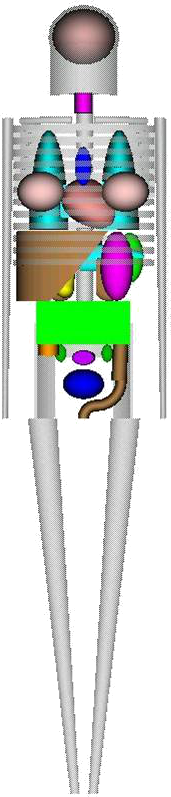
\includegraphics[height=.6\textheight]{imgs/phantom1.png} \hspace{2cm}
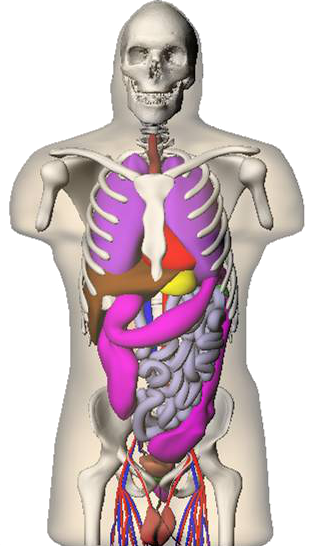
\includegraphics[height=.6\textheight]{imgs/phantom2.png}
\end{center}

\end{frame}

\begin{frame}{From diagnostic to therapy}
\protect\hypertarget{from-diagnostic-to-therapy}{}

\textbf{New times}

\begin{itemize}
\item
  the increasing number of nuclear medicine techniques
\item
  the doses involved in different techniques
\item
  the growth of nuclear medicine use in therapy
\end{itemize}

\vspace{.5cm}

\textbf{Demands} \vspace{.3cm}

\begin{center}
\fbox{\begin{minipage}{20em}
\centering
\textcolor{red}{{\bf more accurate dosimetric assessment} \\ {\bf both in tumor tissues and organs at risk}}
\end{minipage}}
\end{center}

\end{frame}

\begin{frame}{Dosimetric Nuclear Medicine methods}
\protect\hypertarget{dosimetric-nuclear-medicine-methods}{}

\begin{itemize}
\tightlist
\item
  \textbf{S-values}

  \begin{itemize}
  \tightlist
  \item
    \underline{Def:} Mean dose per unit cumulated activity
  \item
    \underline{Res:} Organ, sub-organ, voxel
  \end{itemize}
\item
  \textbf{DPK convolution}

  \begin{itemize}
  \tightlist
  \item
    \underline{Def:} Radial distribution for mean dose around a point
    source
  \item
    \underline{Res:} Voxel
  \end{itemize}
\item
  \textbf{Monte Carlo}

  \begin{itemize}
  \tightlist
  \item
    \underline{Def:} Monte Carlo radiation transport and delivered
    energy simulation
  \item
    \underline{Res:} Organ, sub-organ, voxel
  \end{itemize}
\end{itemize}

\end{frame}

\begin{frame}{Pros \& Cons}
\protect\hypertarget{pros-cons}{}

\begin{itemize}
\tightlist
\item
  \textbf{S-values}

  \begin{itemize}
  \tightlist
  \item
    \underline{Pros:} standardized and fast calculation
  \item
    \underline{Cons:} limited to specified regions, uncertainties can
    reach 30-40\%
  \end{itemize}
\item
  \textbf{DPK convolution}

  \begin{itemize}
  \tightlist
  \item
    \underline{Pros:} fast calculation
  \item
    \underline{Cons:} already not stablished for non-homogeneous media
    \(\leftarrow\) \textcolor{red}{working on it!}
  \end{itemize}
\item
  \textbf{Monte Carlo}

  \begin{itemize}
  \tightlist
  \item
    \underline{Pros:} the most accurate calculation and the only one
    accepted for non-homogeneous media and complex geometries
  \item
    \underline{Cons:} high computational cost \(\leftarrow\)
    \textcolor{red}{working on hacking it!}
  \end{itemize}
\end{itemize}

\end{frame}

\begin{frame}{patient-specific dosimetry?}
\protect\hypertarget{patient-specific-dosimetry}{}

\begin{itemize}
\item
  \textbf{S-values:} only minor corrections can be made
\item
  \textbf{DPK:} possible, limited for some regions (where there are no
  large density changes) and \textcolor{red}{in progress} solved when
  considering DPK performance in non-homogeneous media
\item
  \textbf{Monte Carlo:} the most accurate and precise
\end{itemize}

\end{frame}

\begin{frame}{Organ, sub-organ and voxel level?}
\protect\hypertarget{organ-sub-organ-and-voxel-level}{}

In order to asses 3D patient-specific dosimetry it is desired to
perform:

\begin{itemize}
\item
  sub-organ and/or voxelized resolution
\item
  consider the actual mass/tissue distribution \(\leftarrow\) CT, RMN
\item
  take into account patient-specific real activty distribution
  \(\leftarrow\) SPECT, PET
\end{itemize}

\end{frame}

\begin{frame}{The proposal}
\protect\hypertarget{the-proposal}{}

Design and development of a computational tool devoted to:

\begin{itemize}
\item
  compute dose delivery at voxel (or sub-organ) level with millimetric
  resolution
\item
  consider the actual tissue patient distribution
\item
  use the actual avtivity distribution and its time evolution
\item
  integrate parameters for planar dosimetry nowadays in use
\end{itemize}

\end{frame}

\hypertarget{dosis-an-integrated-system-for-patient-specific-dosimetry-assessment-at-voxel-level}{%
\section{\texorpdfstring{DOSIS: \emph{an integrated system for
patient-specific dosimetry assessment at voxel
level}}{DOSIS: an integrated system for patient-specific dosimetry assessment at voxel level}}\label{dosis-an-integrated-system-for-patient-specific-dosimetry-assessment-at-voxel-level}}

\begin{frame}{DPK assessment}
\protect\hypertarget{dpk-assessment}{}

\begin{itemize}
\item
  performed by Monte Carlo simulations

  \begin{itemize}
  \tightlist
  \item
    photons, positrons and electrons \(\leftarrow\) PENELOPE
  \item
    alpha and others \(\leftarrow\) FLUKA
    \textcolor{red}{in progress...}
  \end{itemize}
\item
  a model for estimating electrons DPK for different tissues have been
  developed\footnote{P. Pérez {\it et al.} Int. Journ. of Nucl. Med. Res. 3:45-55, 2016.}
\item
  voxelized kernels generated from radial distributions obtained from
  Monte Carlo
\item
  capable of loading information from dual imaging techniques like
  PET-CT, SPECT-CT or SPECT-RMN
\end{itemize}

\end{frame}

\begin{frame}{DPK MC calculated results}
\protect\hypertarget{dpk-mc-calculated-results}{}

\begin{figure}
\centering
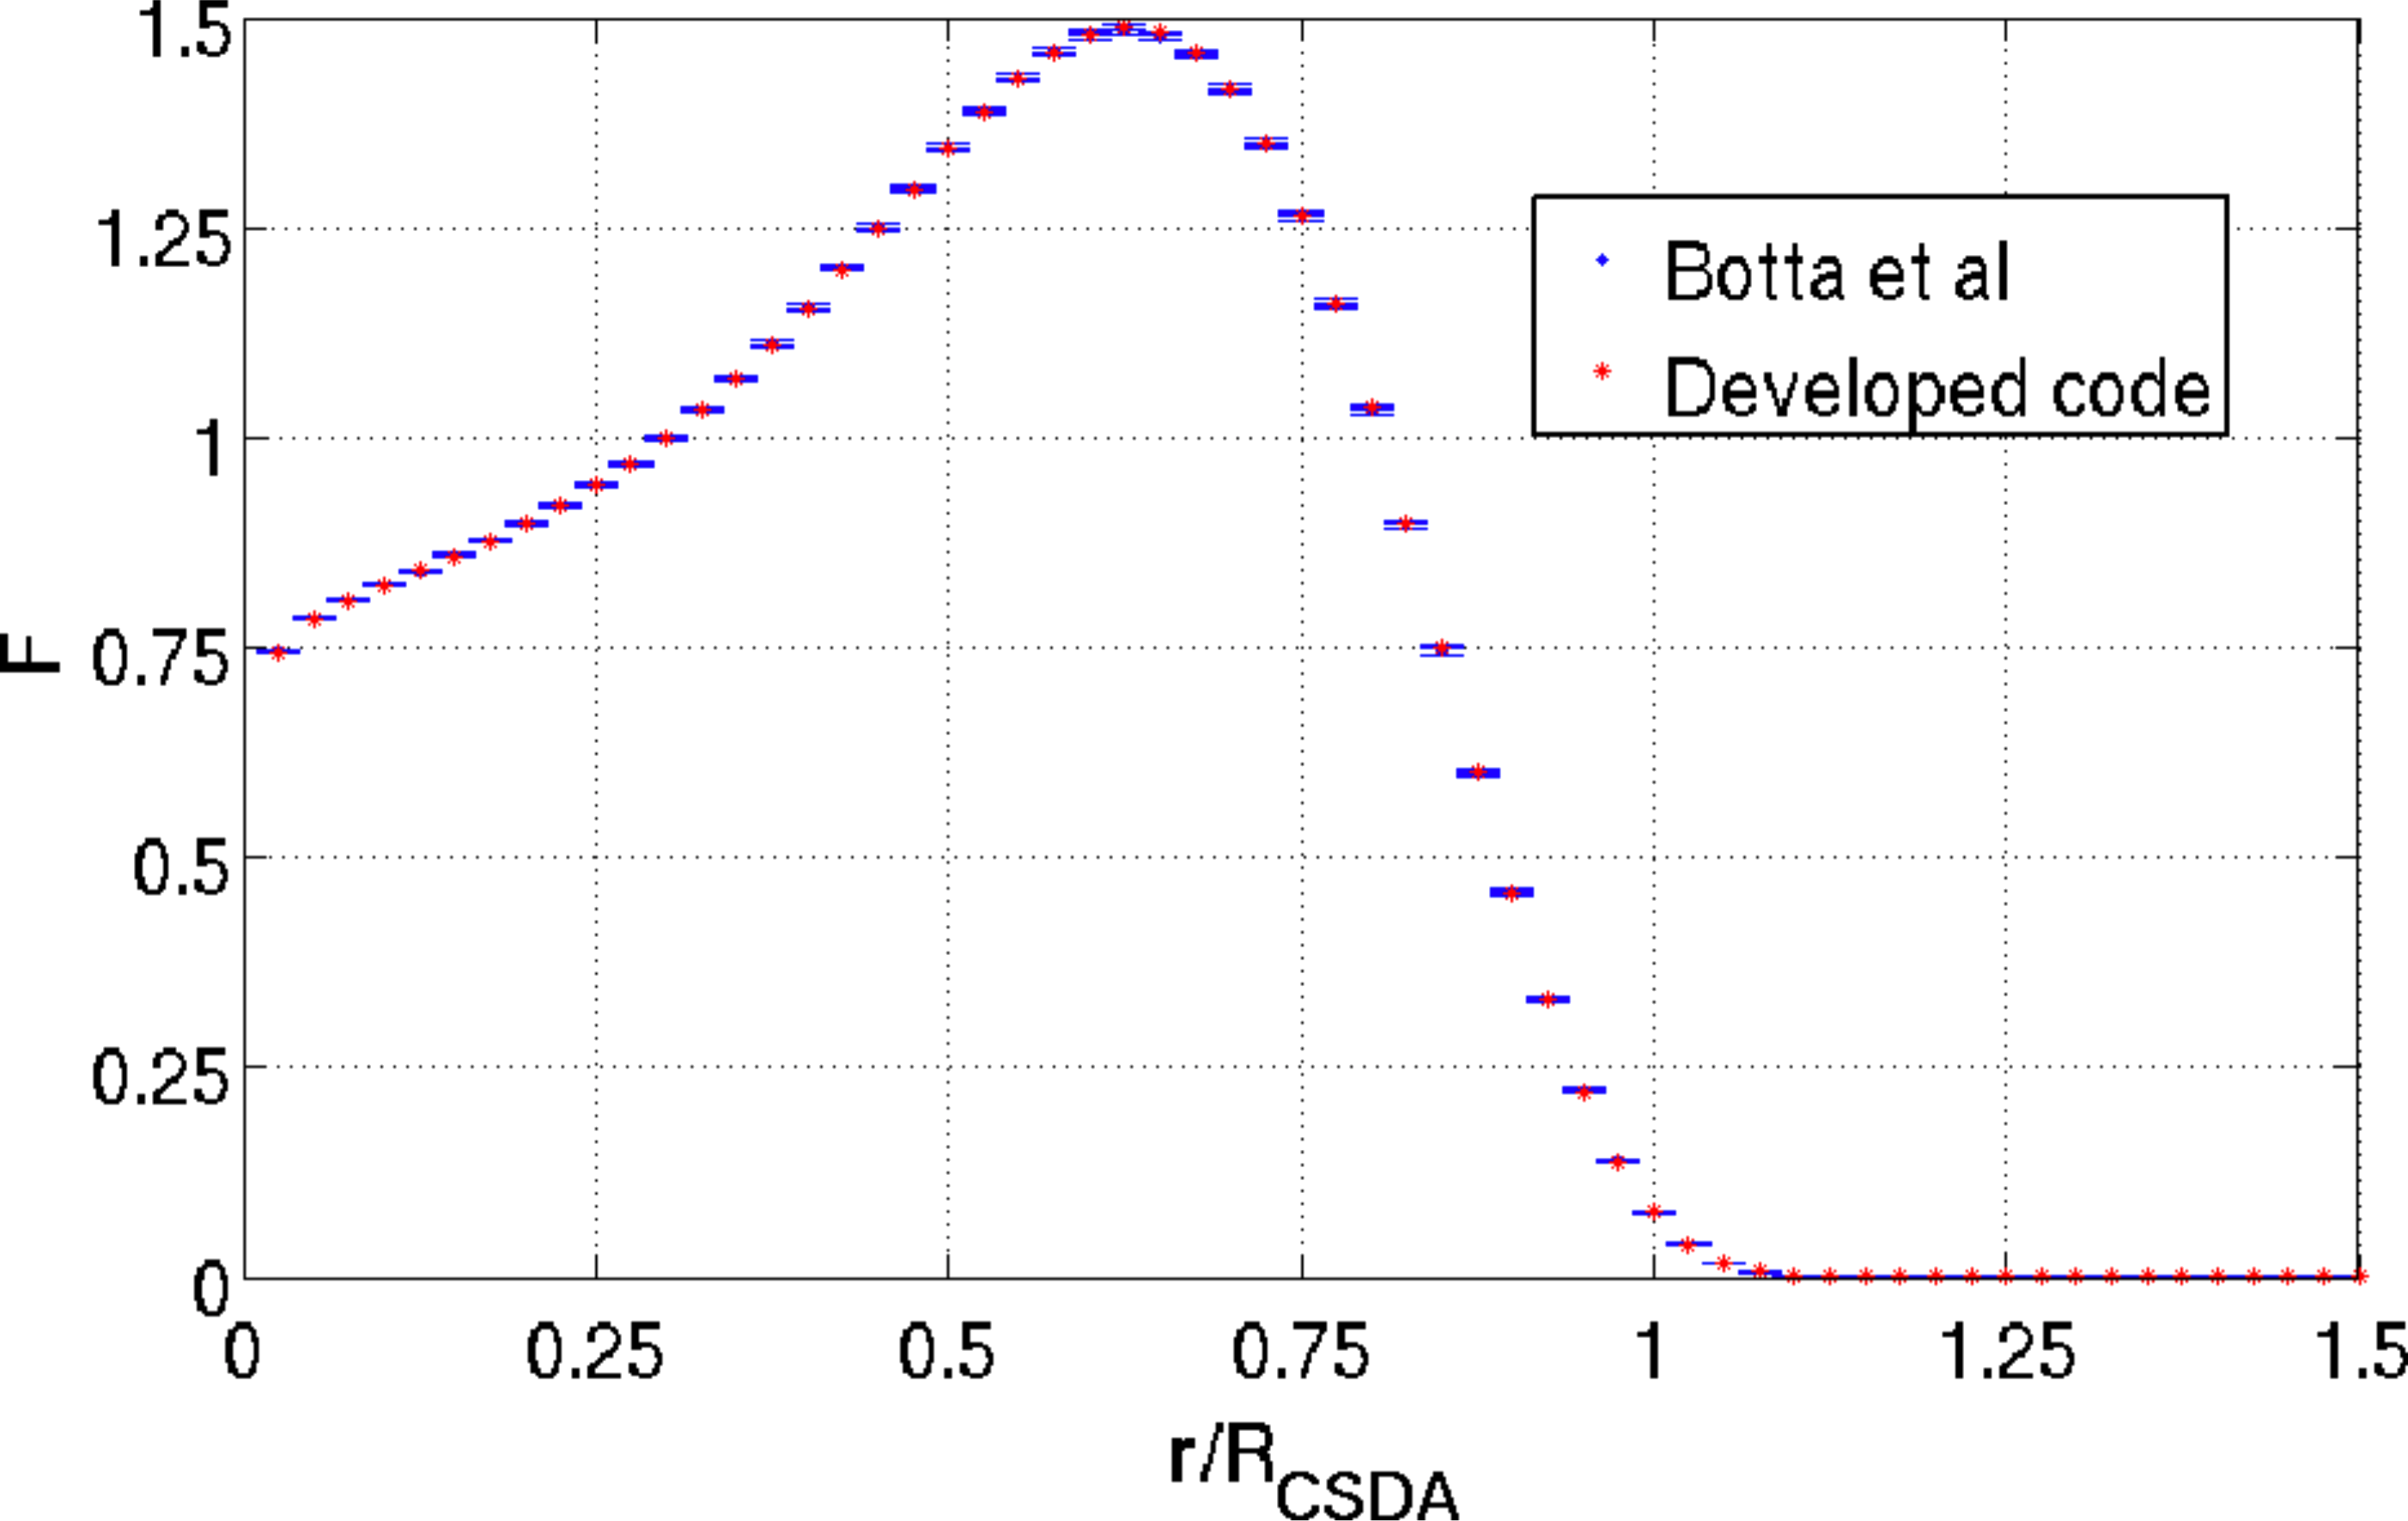
\includegraphics[height=.31\textwidth]{imgs/dpk_validation.png}
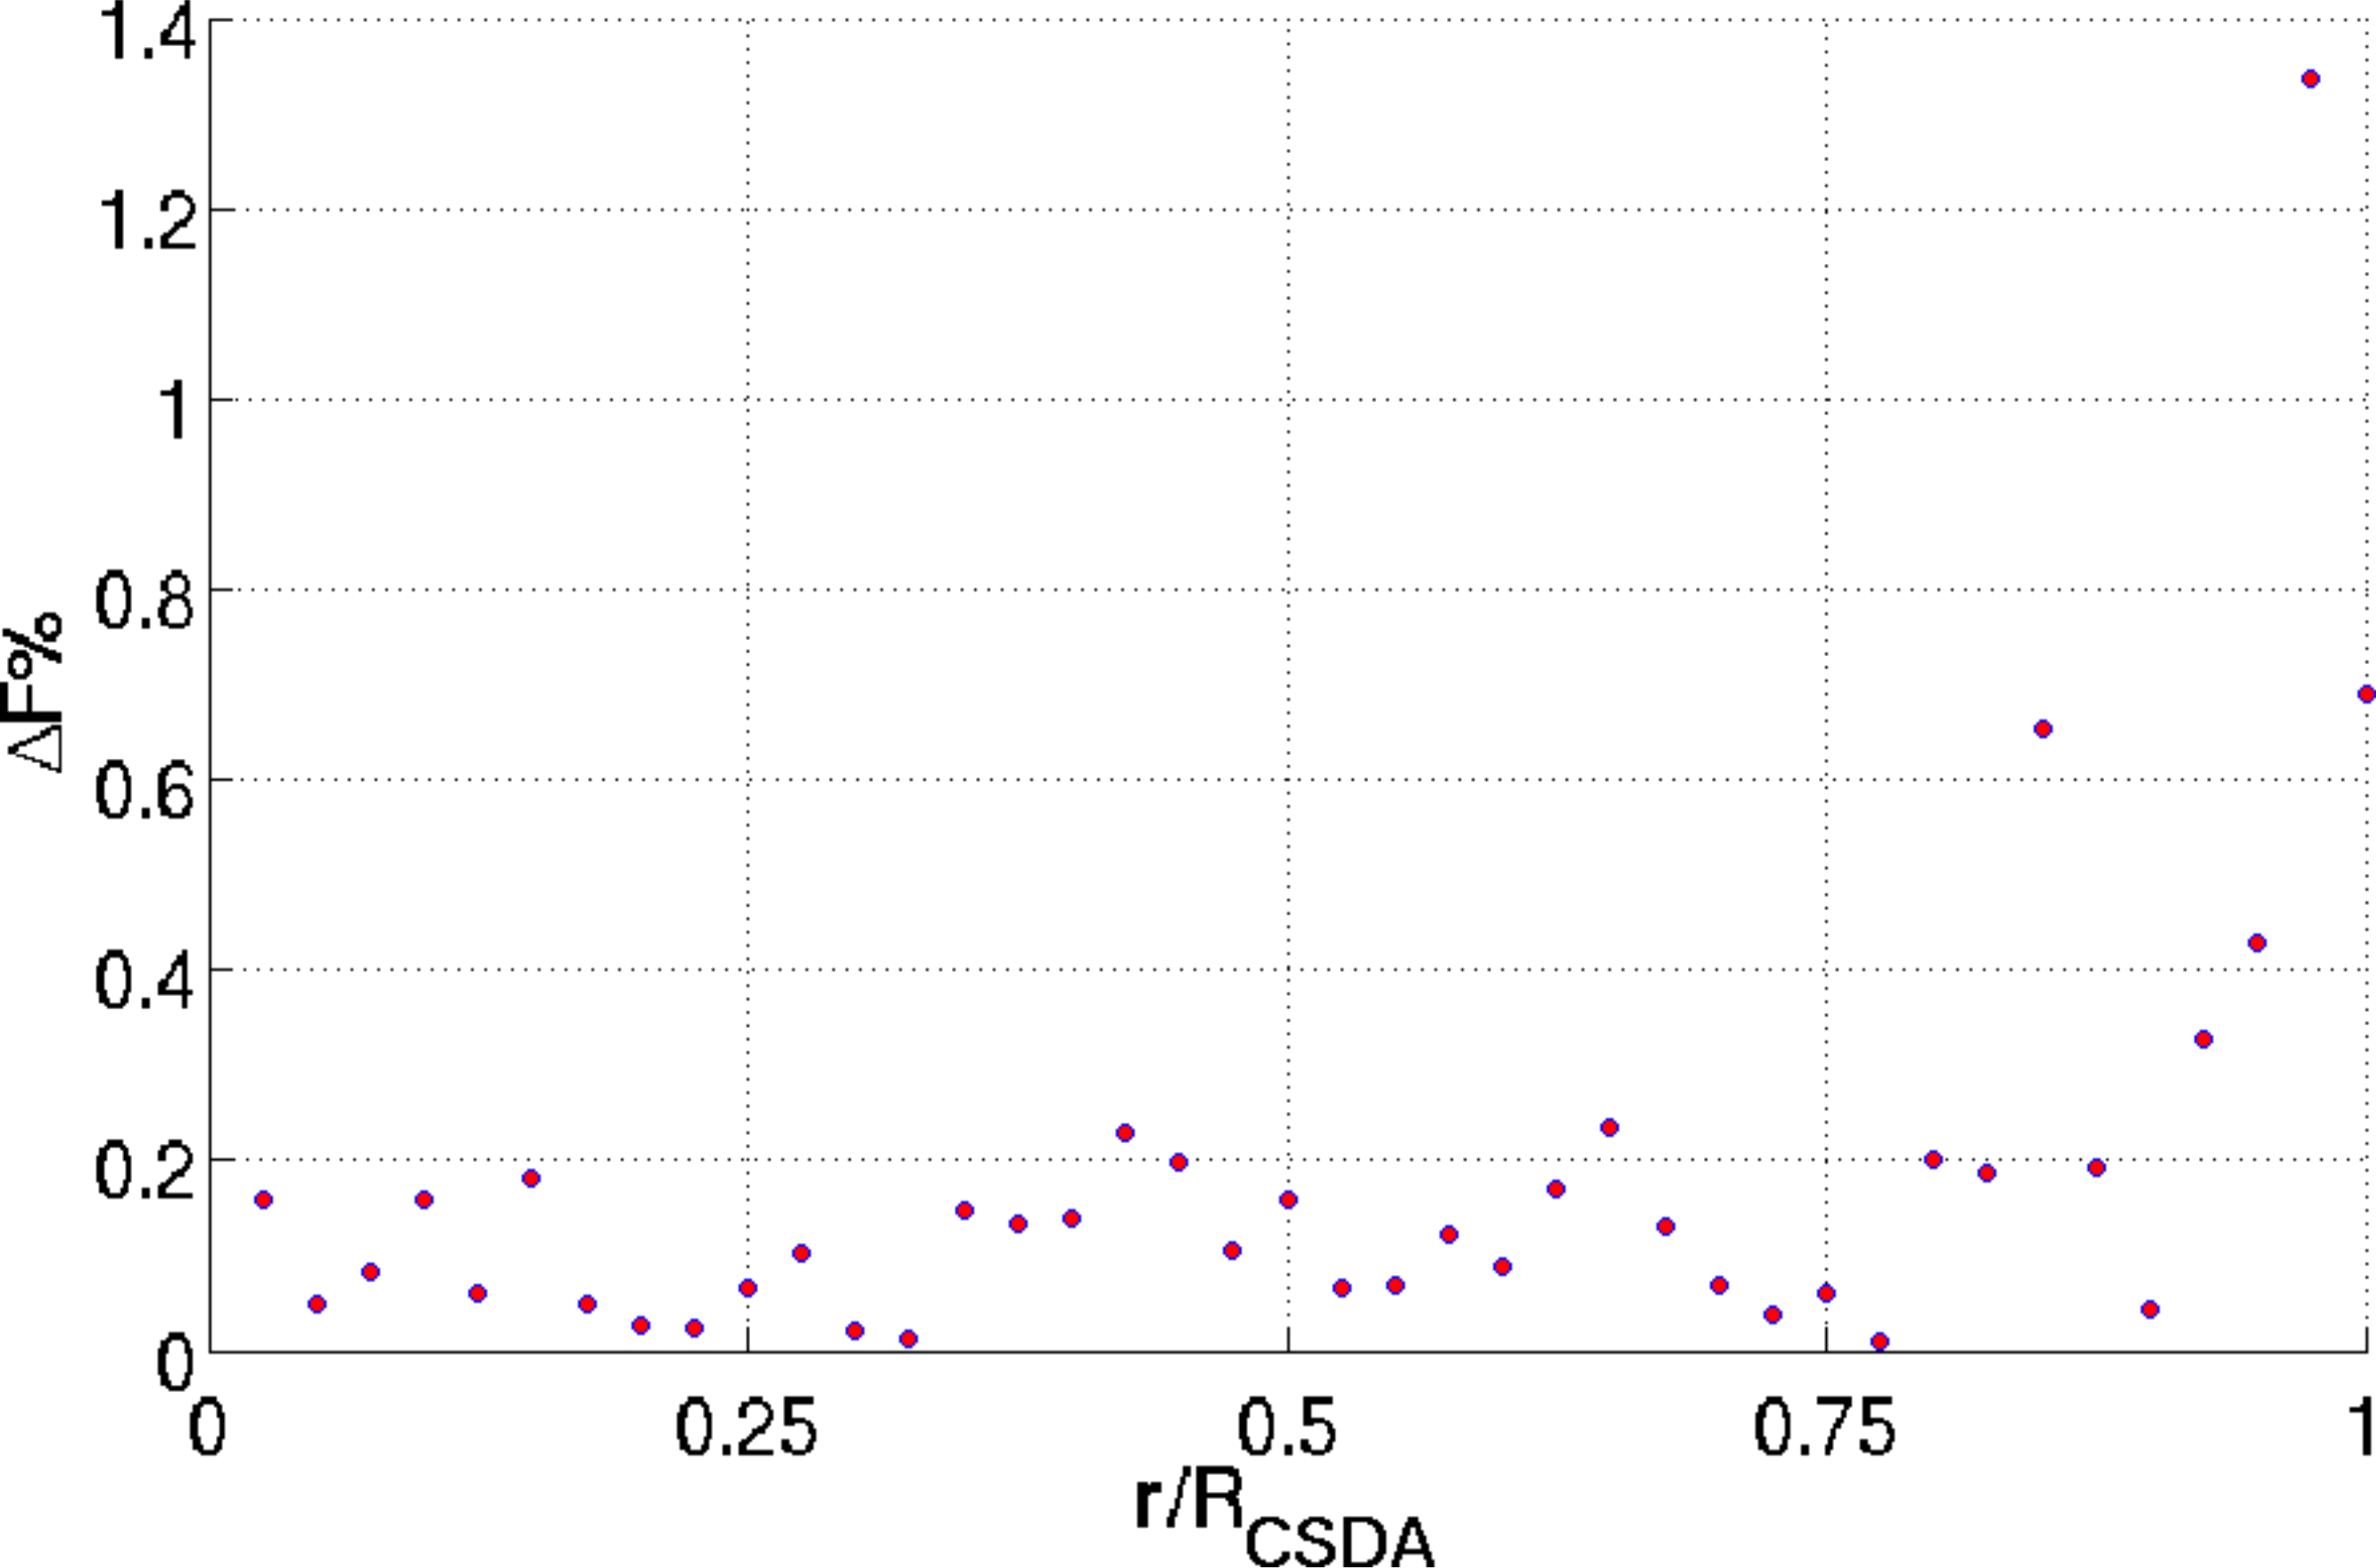
\includegraphics[height=.31\textwidth]{imgs/dpk_validation_err.png}
\end{figure}

sDPK (F) calculated compared with published
data\footnote{Botta et al. Med. Phys. 38(7):3944-3954.} (left) and
uncertainties involved (right)

\end{frame}

\begin{frame}{DPK MC calculated results}
\protect\hypertarget{dpk-mc-calculated-results-1}{}

\begin{figure}
\centering
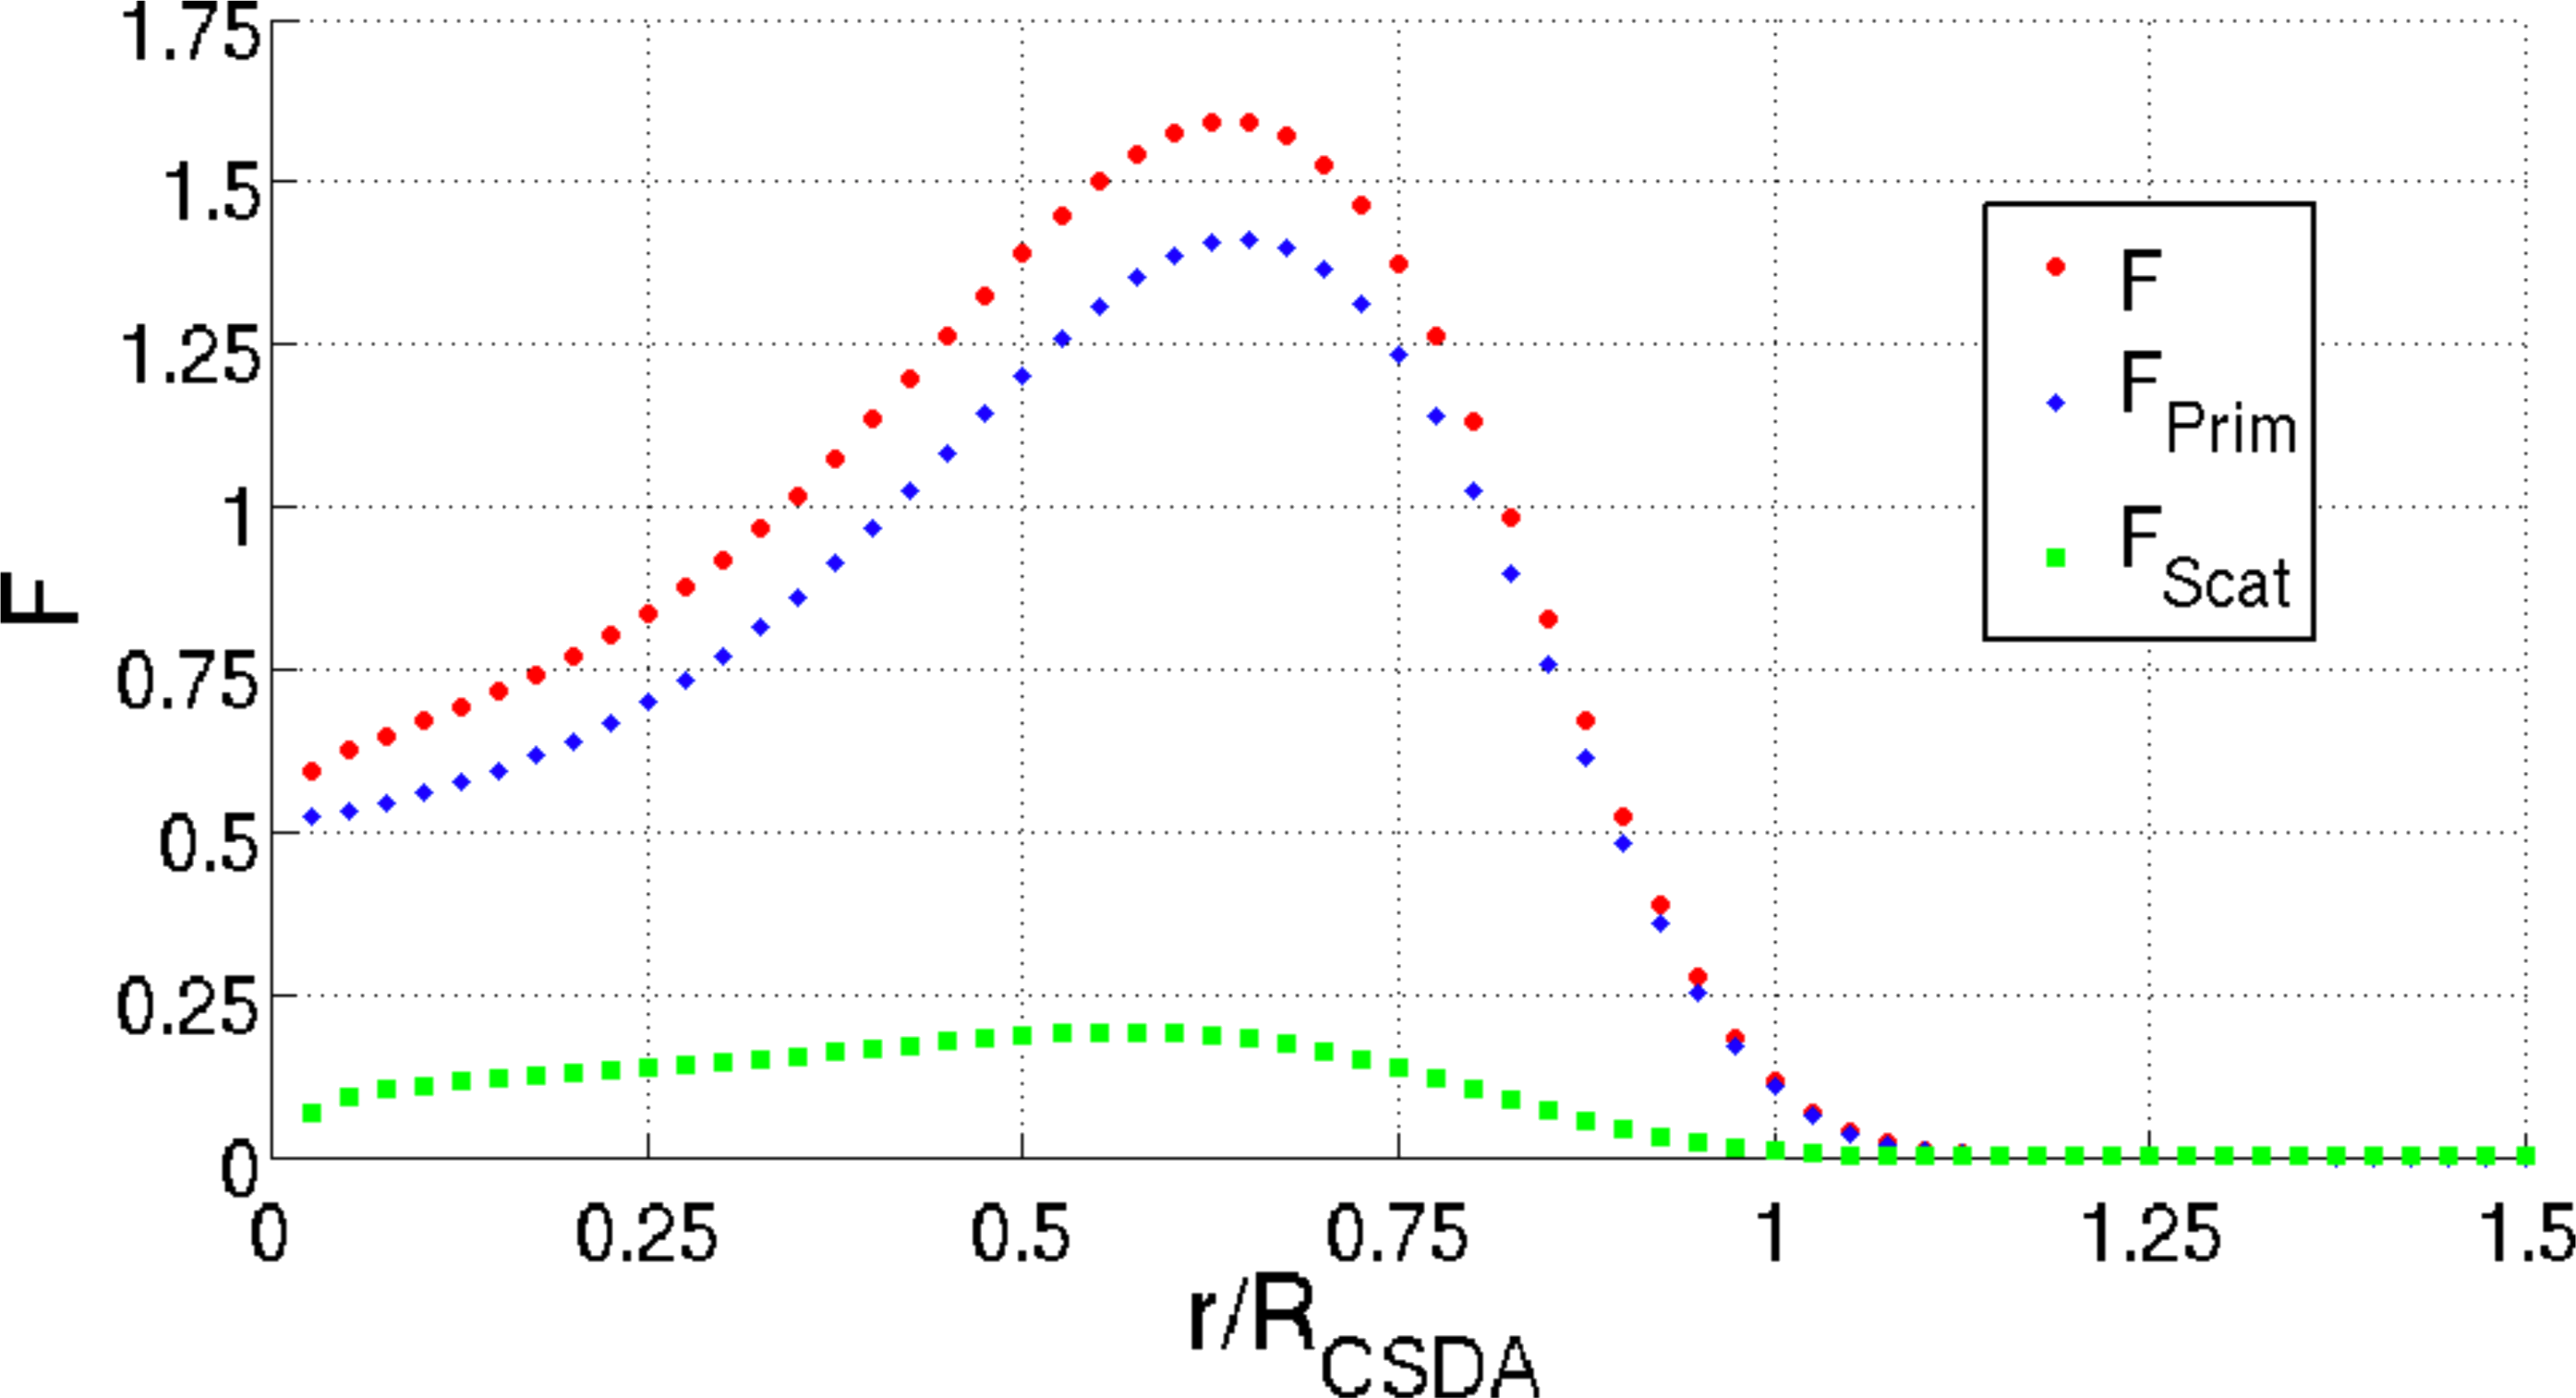
\includegraphics[height=.3\textwidth]{imgs/dpk_discriminacion.png}
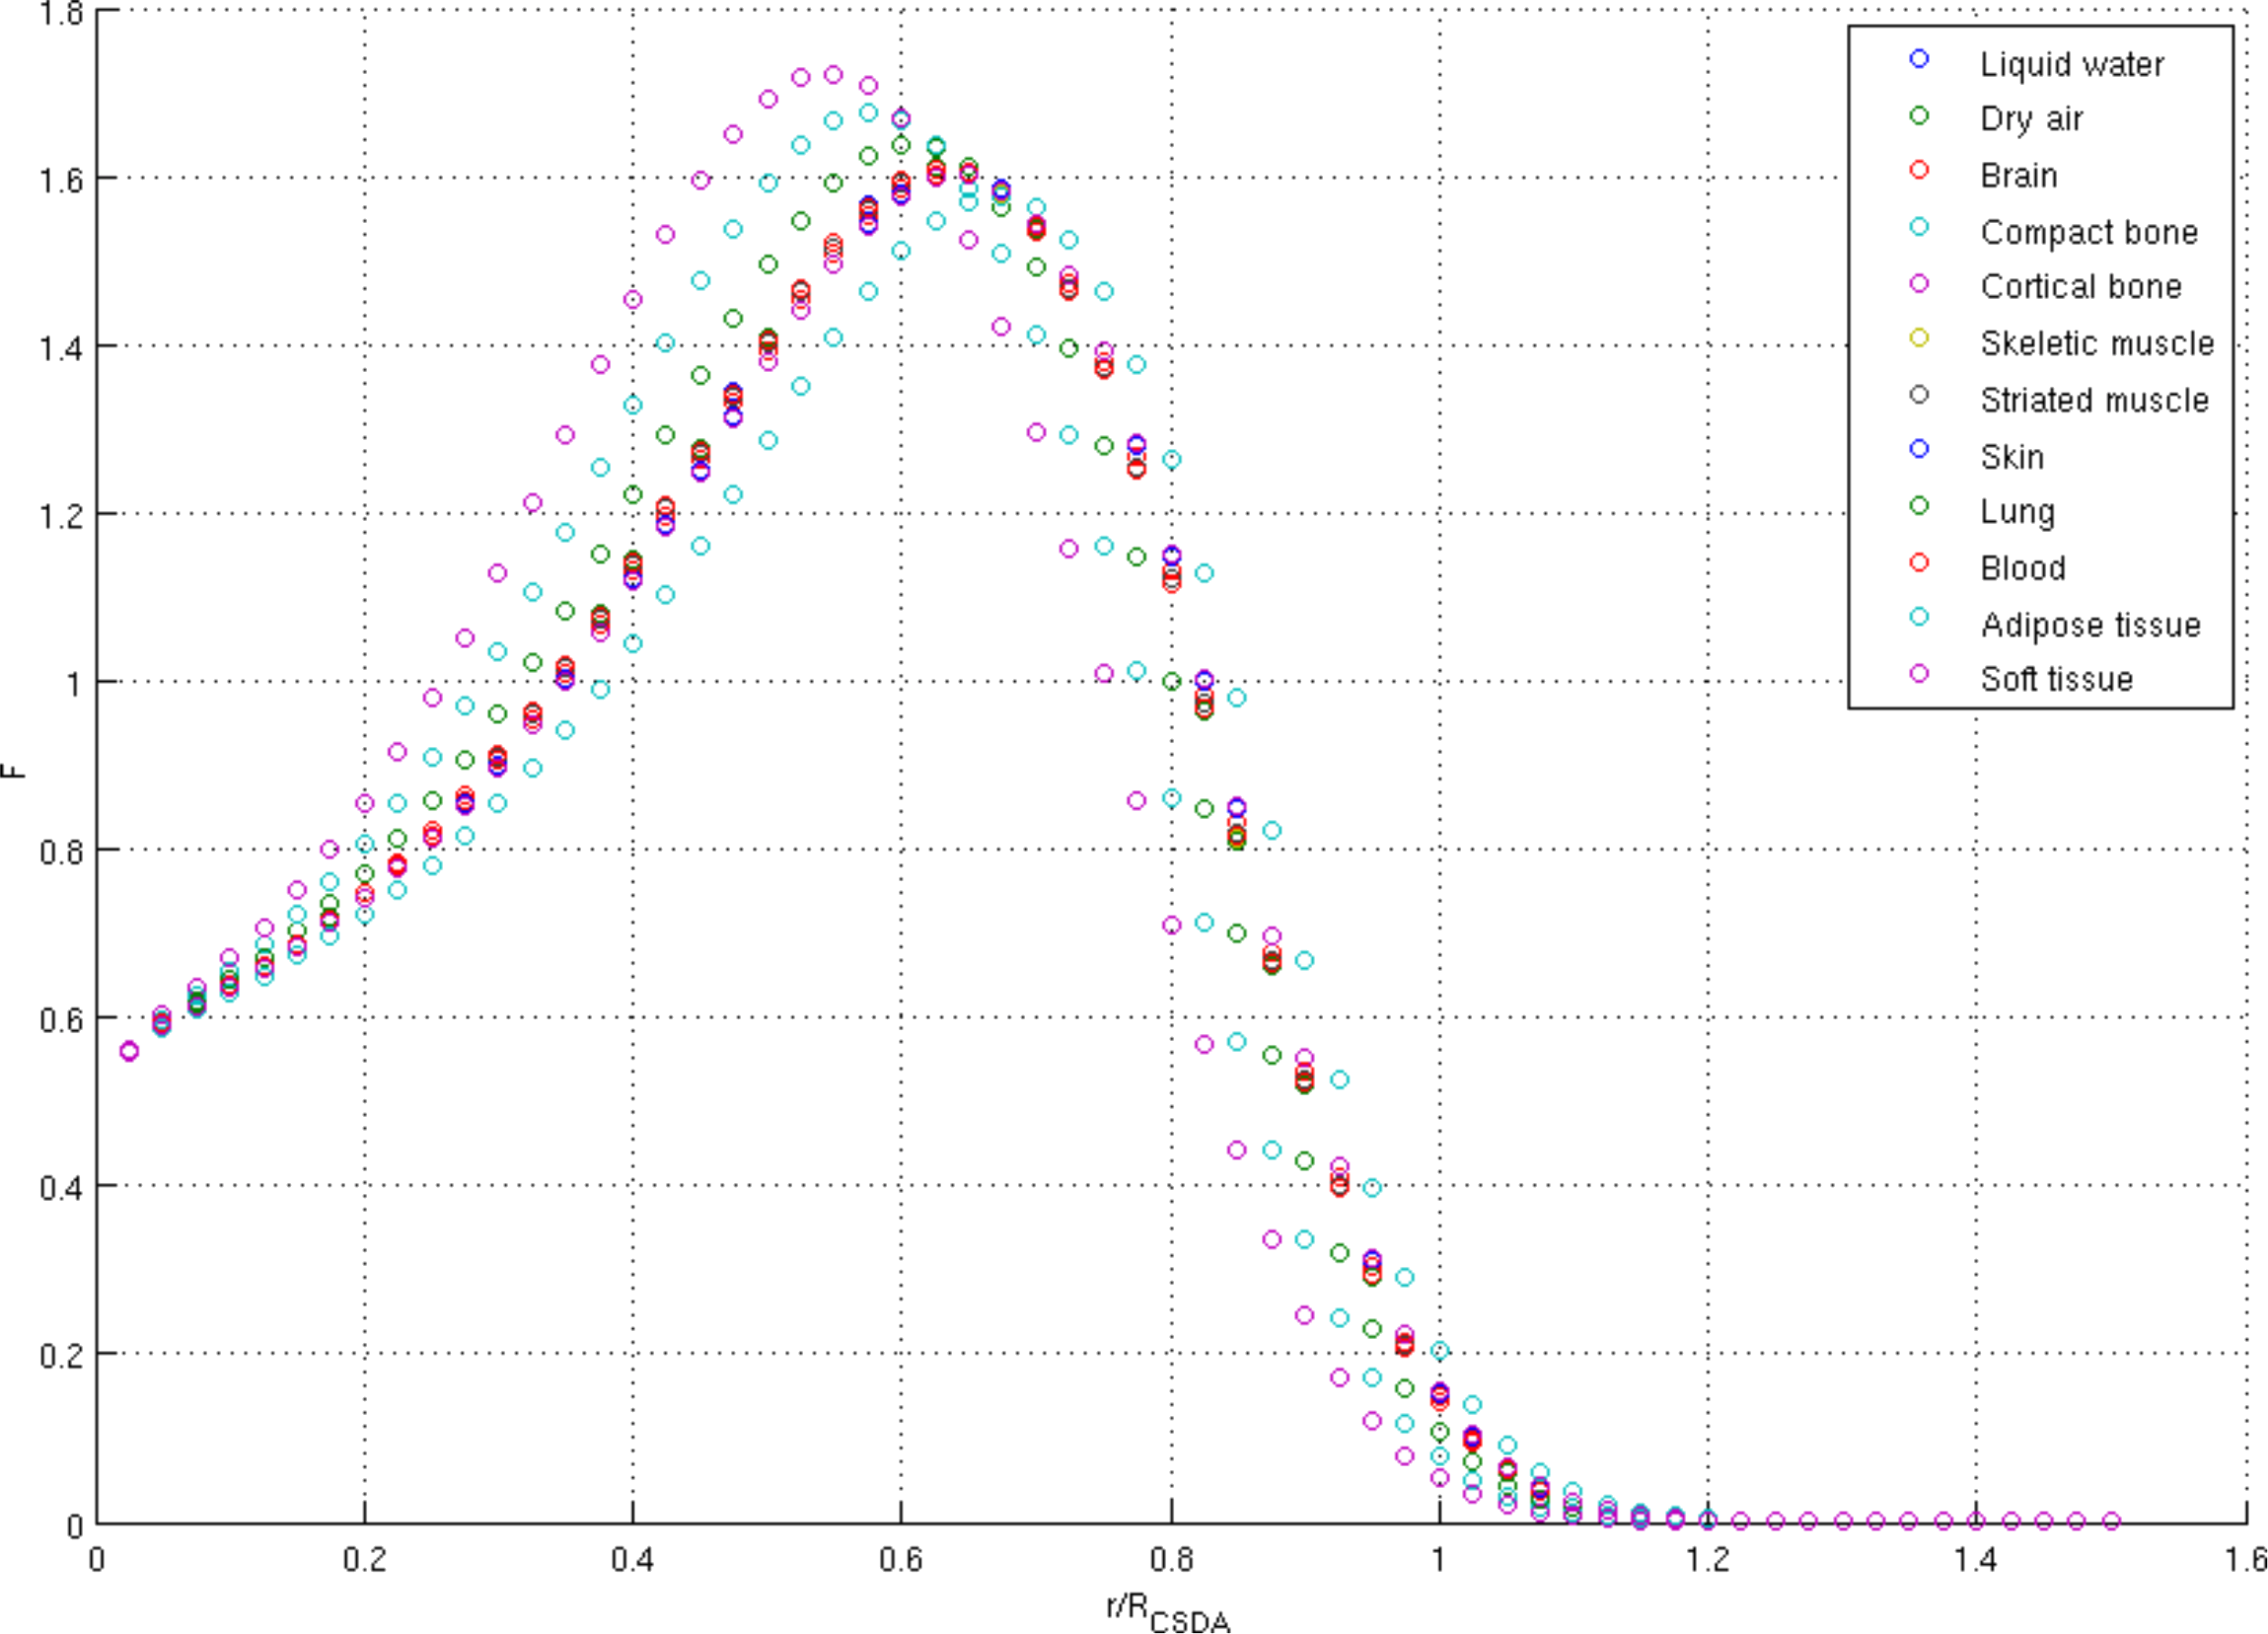
\includegraphics[height=.3\textwidth]{imgs/dpk_tissues.png}
\end{figure}

sDPK (F) calculated discriminating primary and scattering contributions
(left) and for different tissues (right)

\end{frame}

\begin{frame}{Application to internal dosimetry}
\protect\hypertarget{application-to-internal-dosimetry}{}

\textbf{Voxel level dosimetry with DPK convolution}

\begin{itemize}
\item
  Activity distribution can be considered as an array of point sources
\item
  Deposite dose distribution can be calculated by means of integration
  of all of these sources
\item
  This can be made by the convolution technique
\end{itemize}

\begin{equation}
D(\vec{r}) = \mathbb{K}_{D}(\vec{r}) \ast \mathbb{A}_{cum}(\vec{r}) = \int_{-\infty}^{\infty} \mathbb{K}_{D}(\vec{r'}) \mathbb{A}_{cum}(\vec{r} - \vec{r'}) d\vec{r'}
\end{equation}

\end{frame}

\begin{frame}{Background theory}
\protect\hypertarget{background-theory}{}

\textbf{Voxelizing}

\begin{itemize}
\item
  Defining \(\mathcal{K}_D(i,j,k)\) and \(\mathcal{A}_{cum}(i,j,k)\) as
  \(\mathbb{K}_{D}(\vec{r})\) and \(\mathbb{A}_{cum}(\vec{r})\) in 3D
  voxelized geometry
\item
  Using Fourier Transform properties and convolution technique
\item
  Dose \(D(\vec{r})\) results
\end{itemize}

\begin{equation}
D(\vec{r}) = \mathbb{F}^{-1}\{\mathbb{F}\{\mathcal{K}_{D}(i,j,k) \cdot \mathcal{A}_{cum}(i,j,k)\}\}
\end{equation}

And both Matlab and Python (among others) provide libraries to a fast
solve of this equation through Fast Fourier Transform algorithm.

\end{frame}

\hypertarget{graphical-user-interface}{%
\section{Graphical User Interface}\label{graphical-user-interface}}

\begin{frame}{Chartflow}
\protect\hypertarget{chartflow}{}

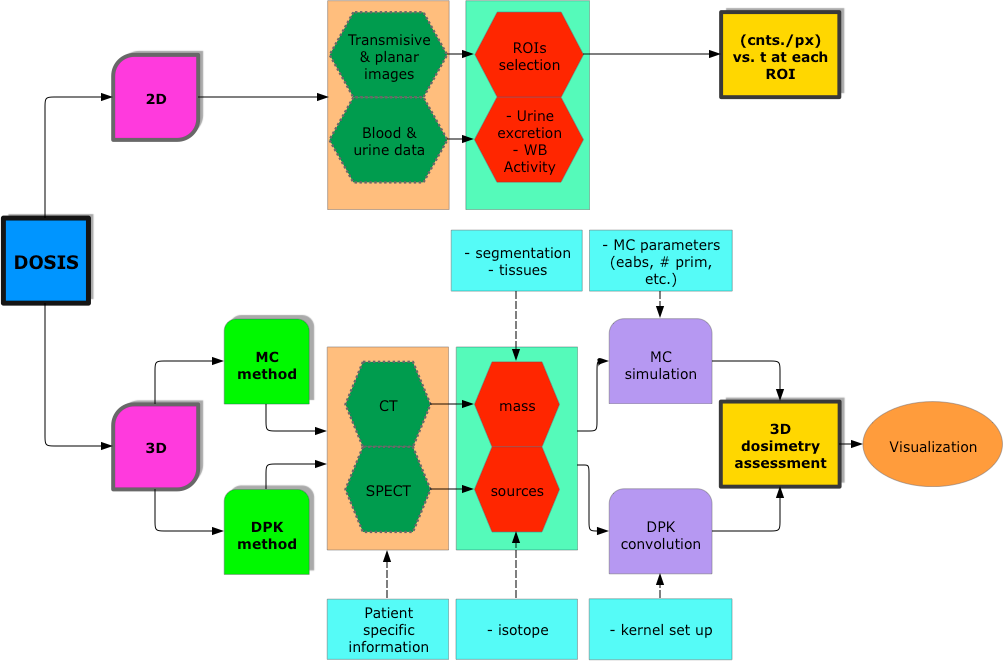
\includegraphics{imgs/dosis-chartflow.png}

\end{frame}

\begin{frame}{Planar dosimetry chartflow}
\protect\hypertarget{planar-dosimetry-chartflow}{}

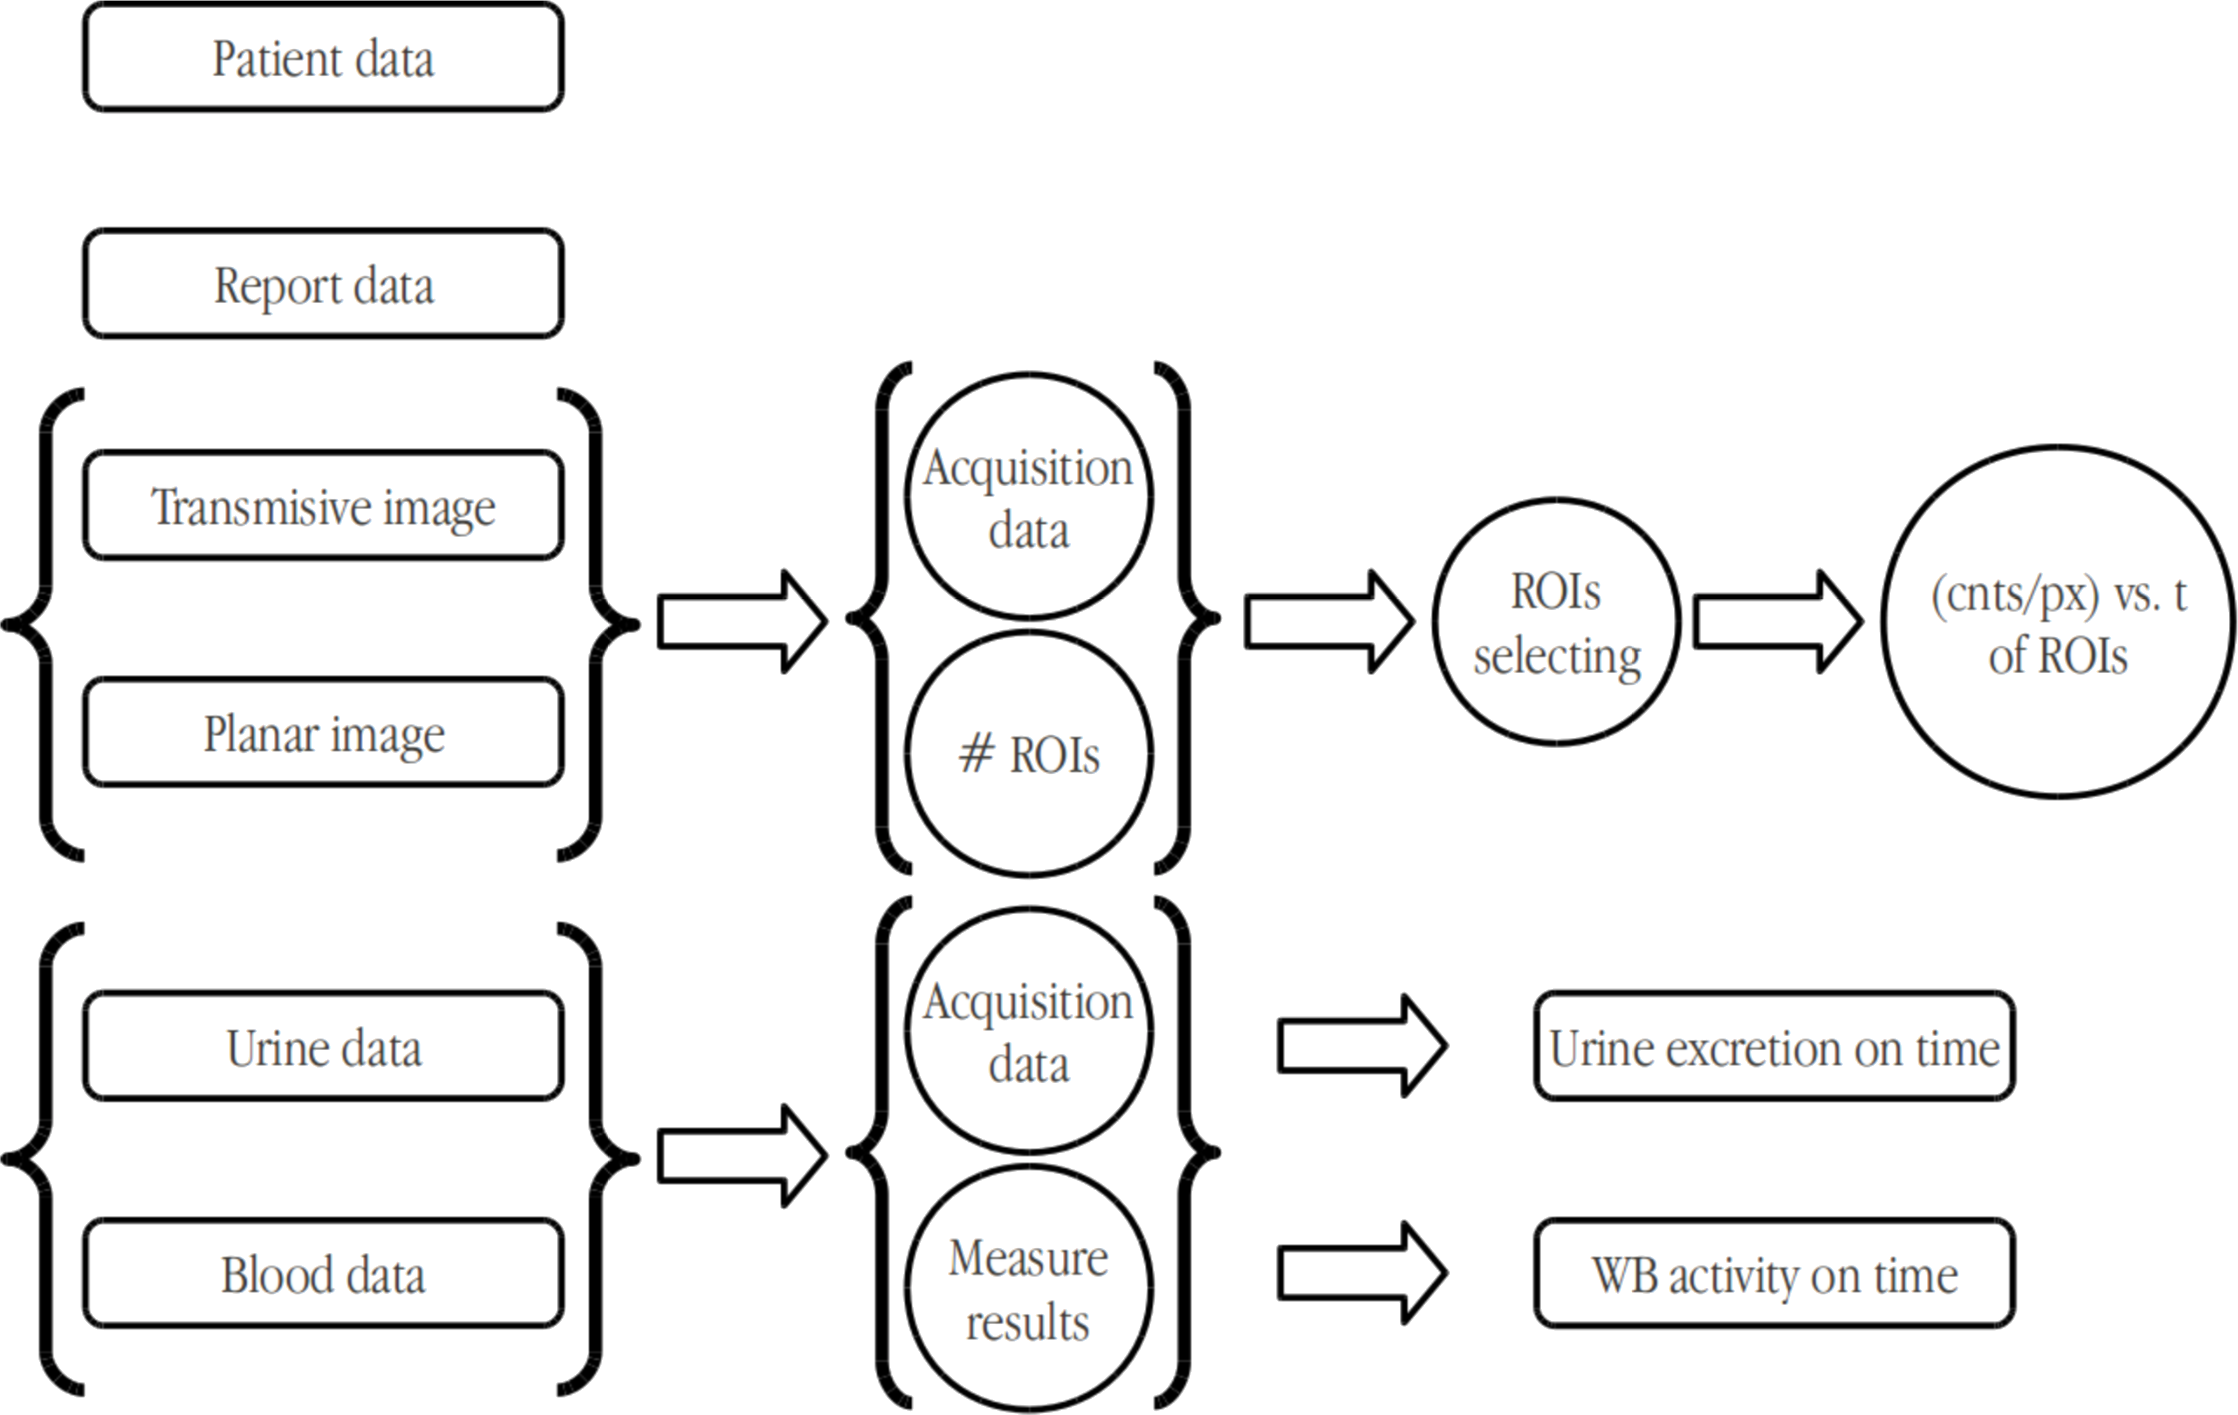
\includegraphics{imgs/planar-chartflow.png}

\end{frame}

\begin{frame}{Planar dosimetry GUI: \emph{main}}
\protect\hypertarget{planar-dosimetry-gui-main}{}

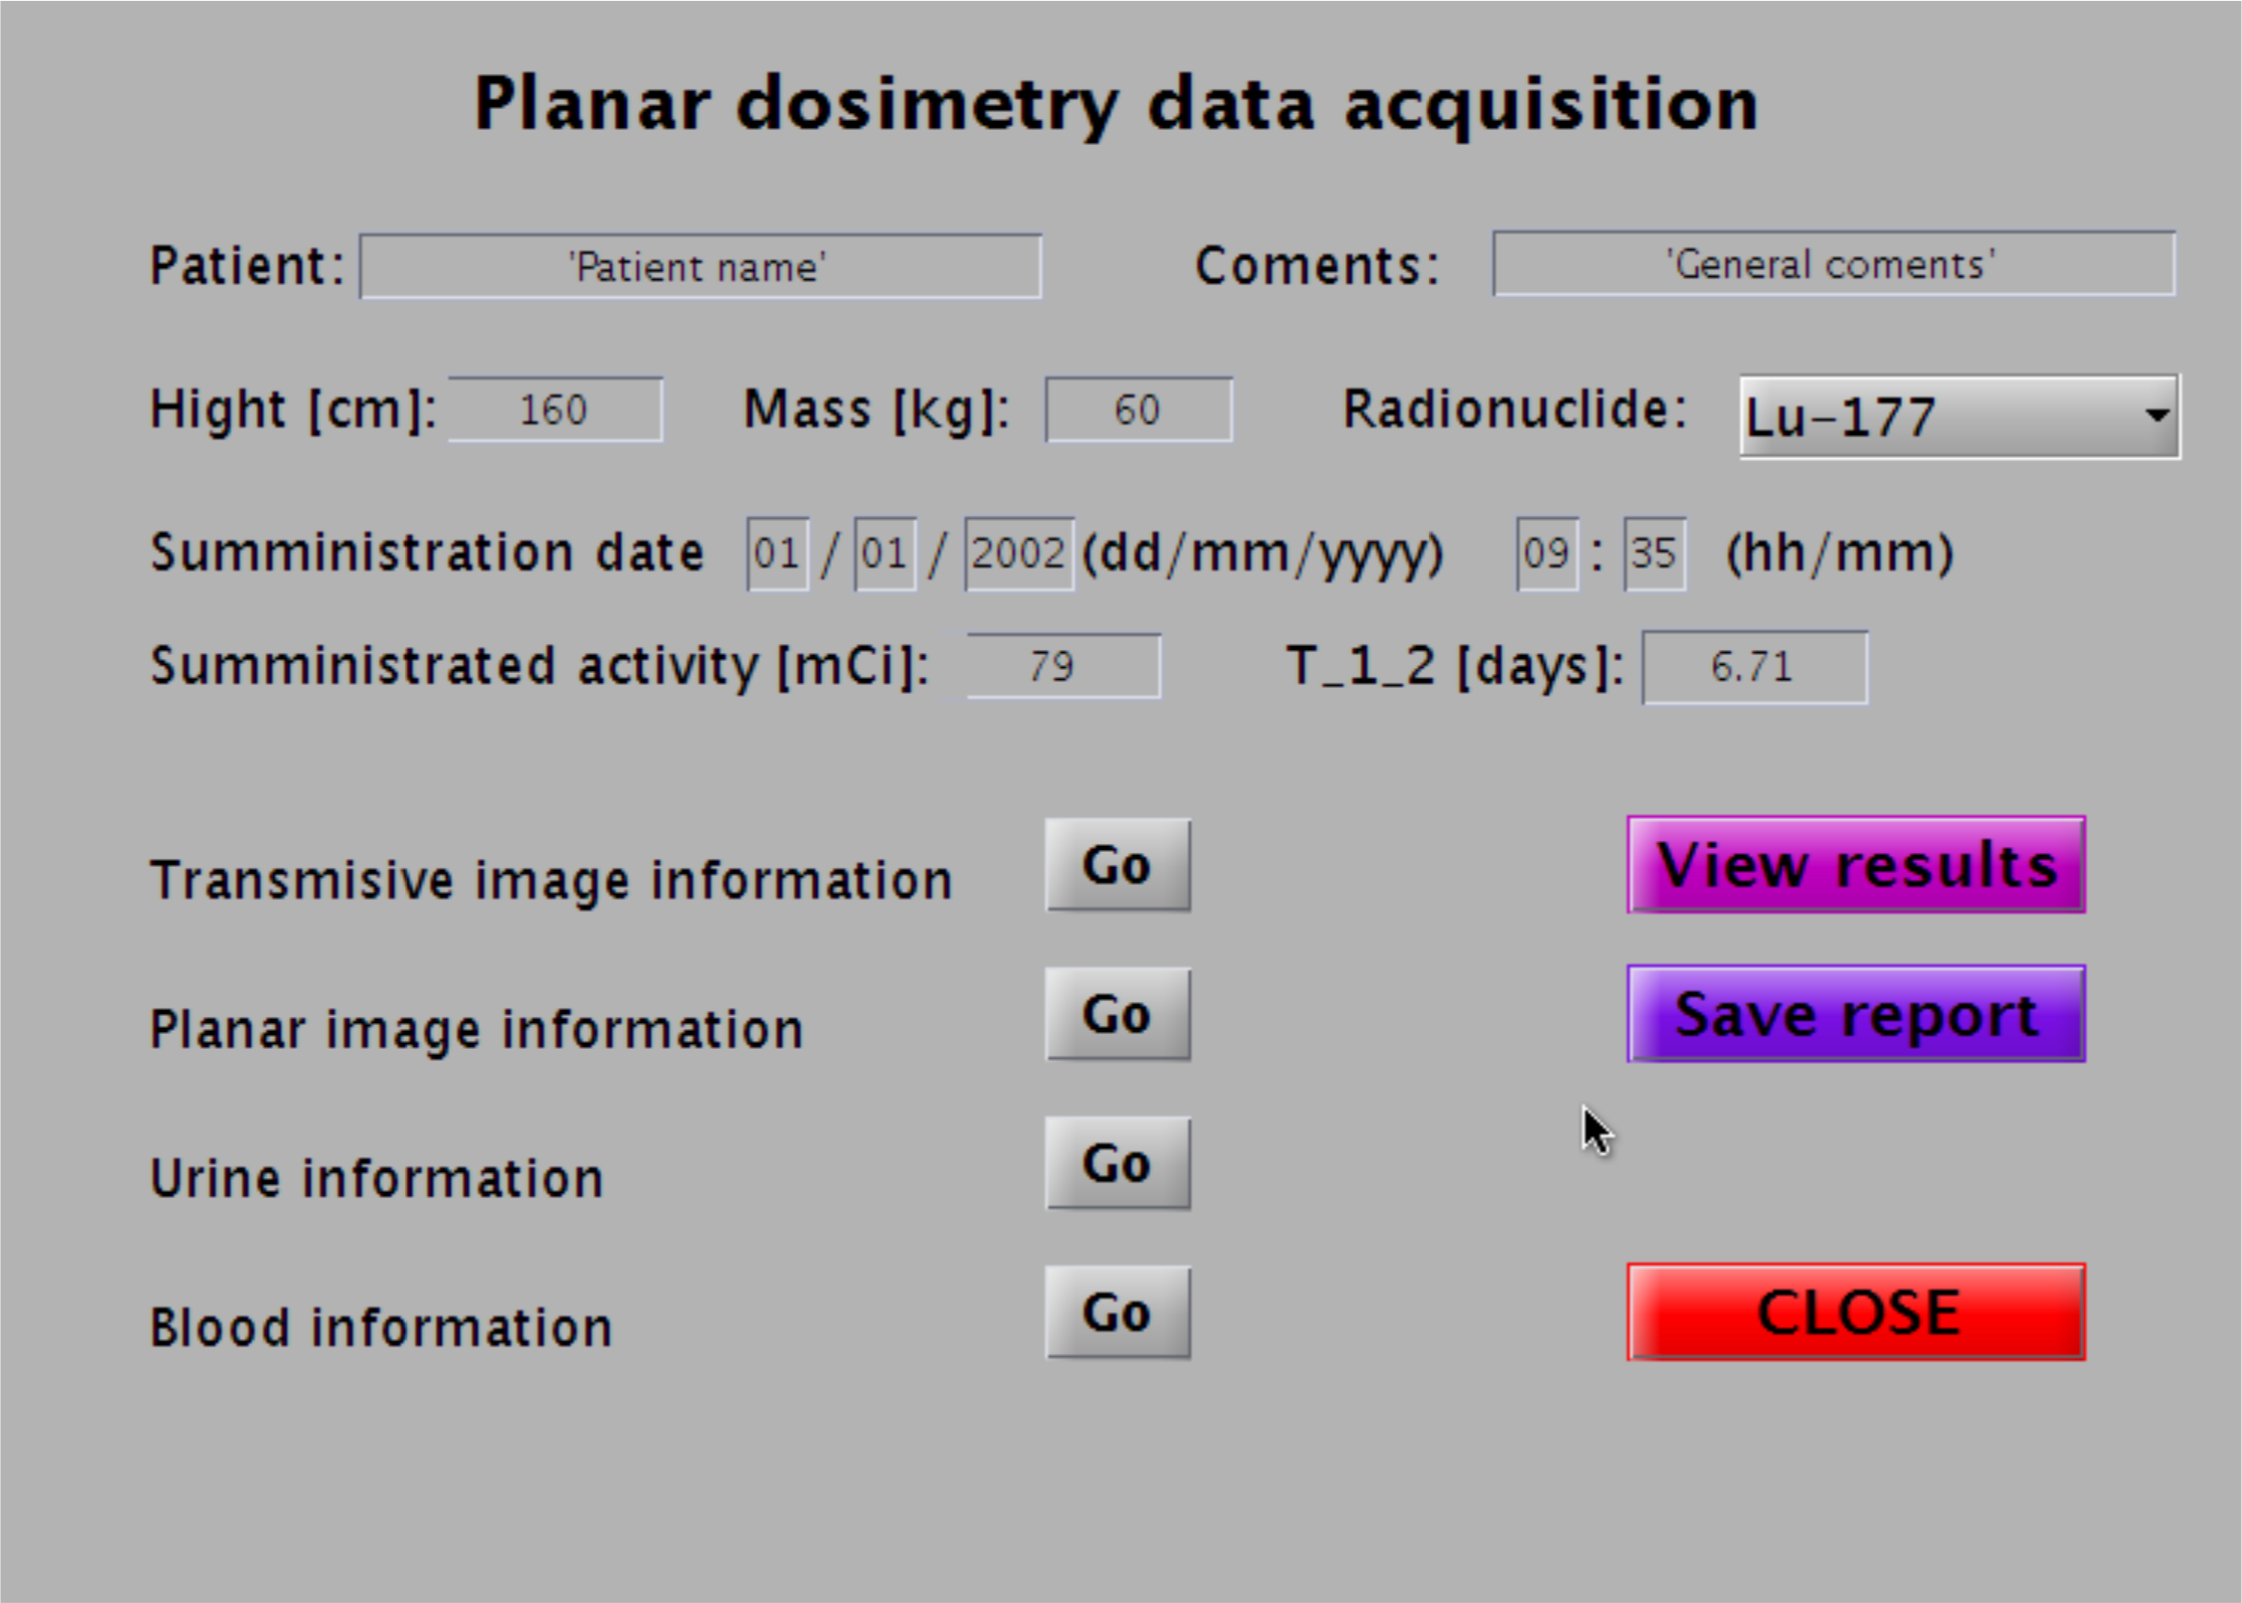
\includegraphics{imgs/planar-gui.png}

\end{frame}

\begin{frame}{Planar dosimetry GUI: \emph{rois}}
\protect\hypertarget{planar-dosimetry-gui-rois}{}

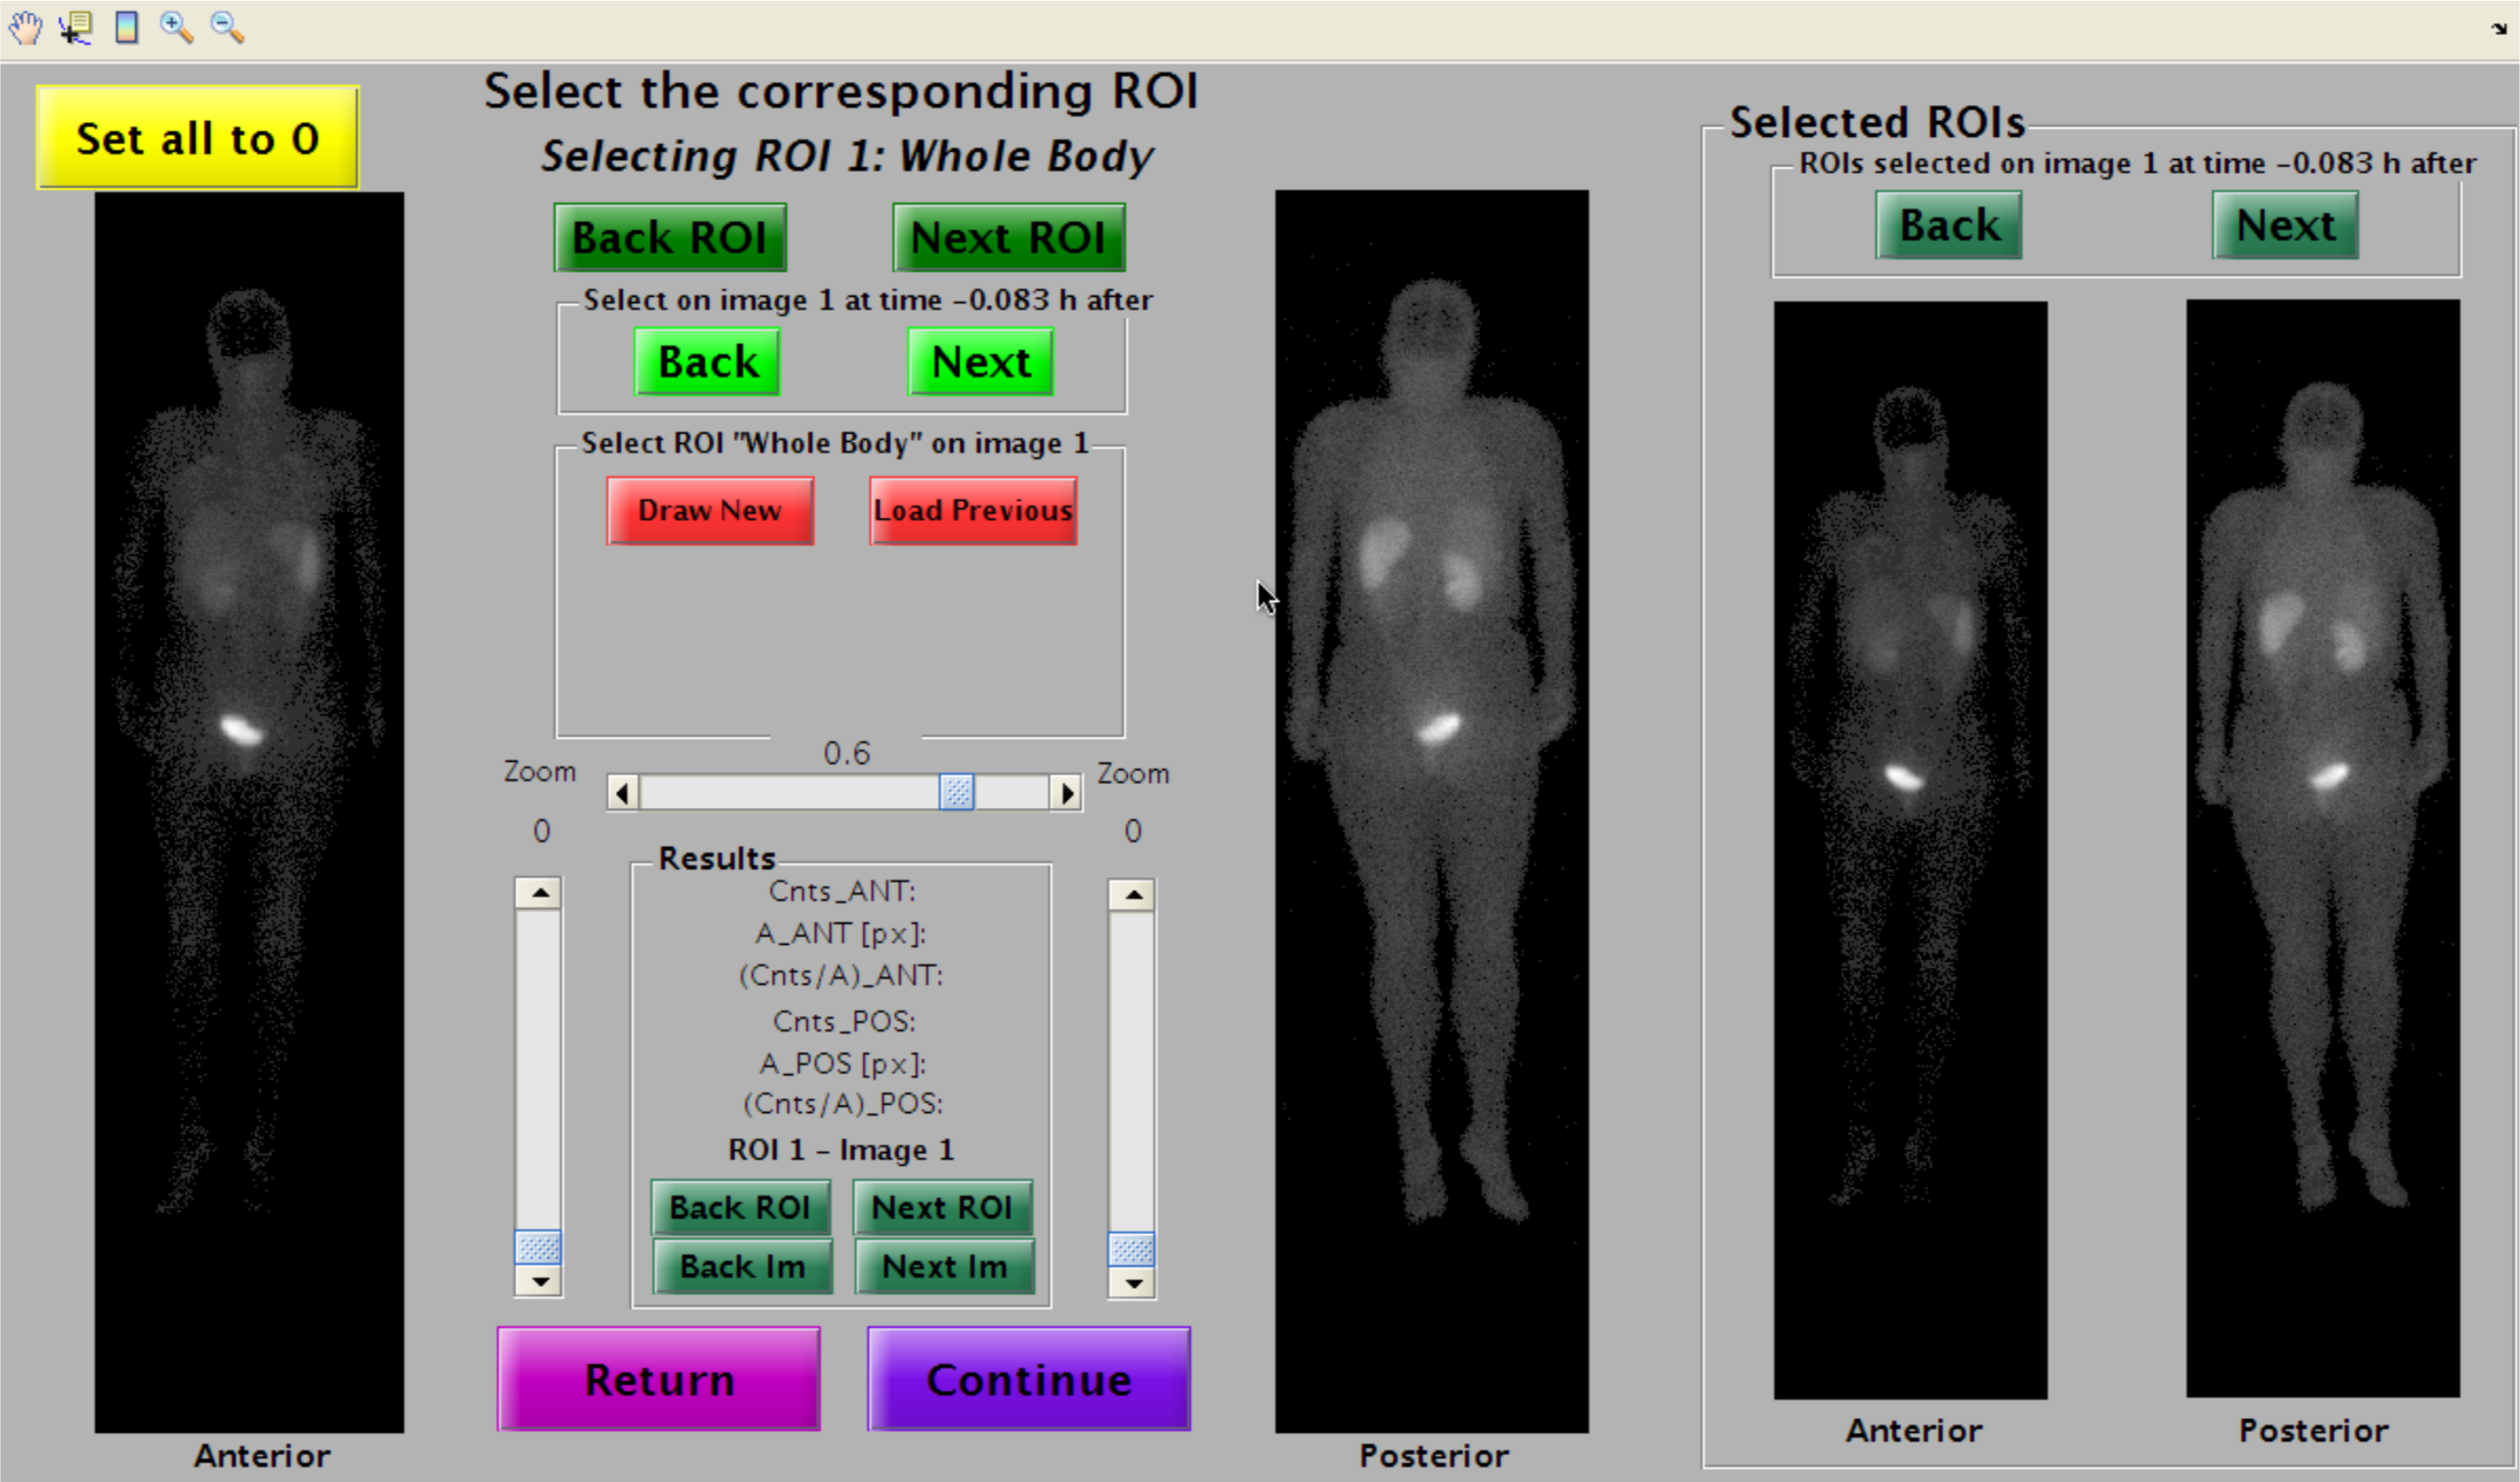
\includegraphics{imgs/planar-rois.png}

\end{frame}

\begin{frame}{Planar dosimetry GUI: \emph{whole body}}
\protect\hypertarget{planar-dosimetry-gui-whole-body}{}

\begin{center}
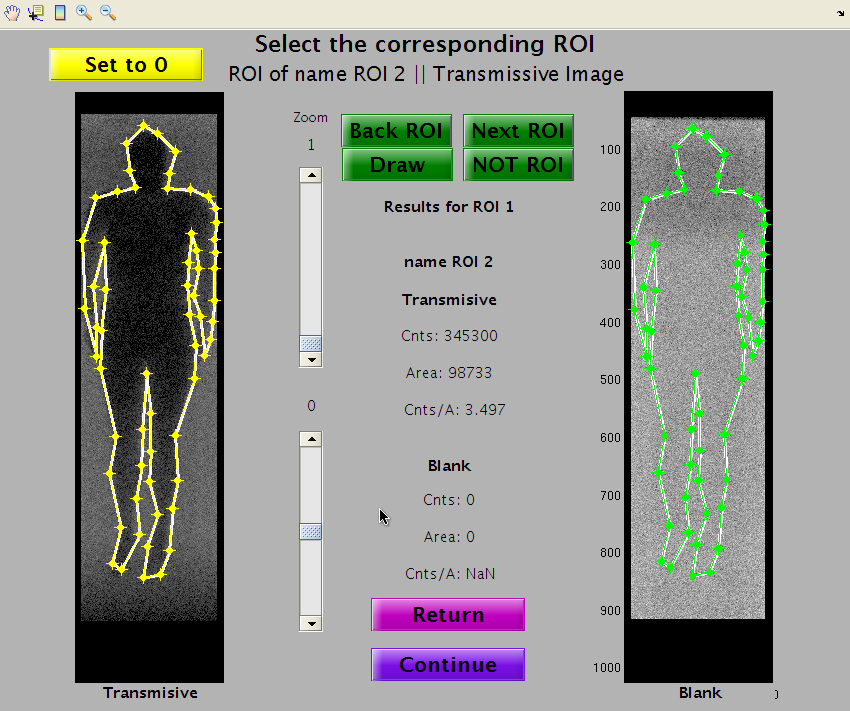
\includegraphics[height=.8\textheight]{imgs/planar-wb.png}
\end{center}

\end{frame}

\begin{frame}{Planar dosimetry GUI: \emph{curves}}
\protect\hypertarget{planar-dosimetry-gui-curves}{}

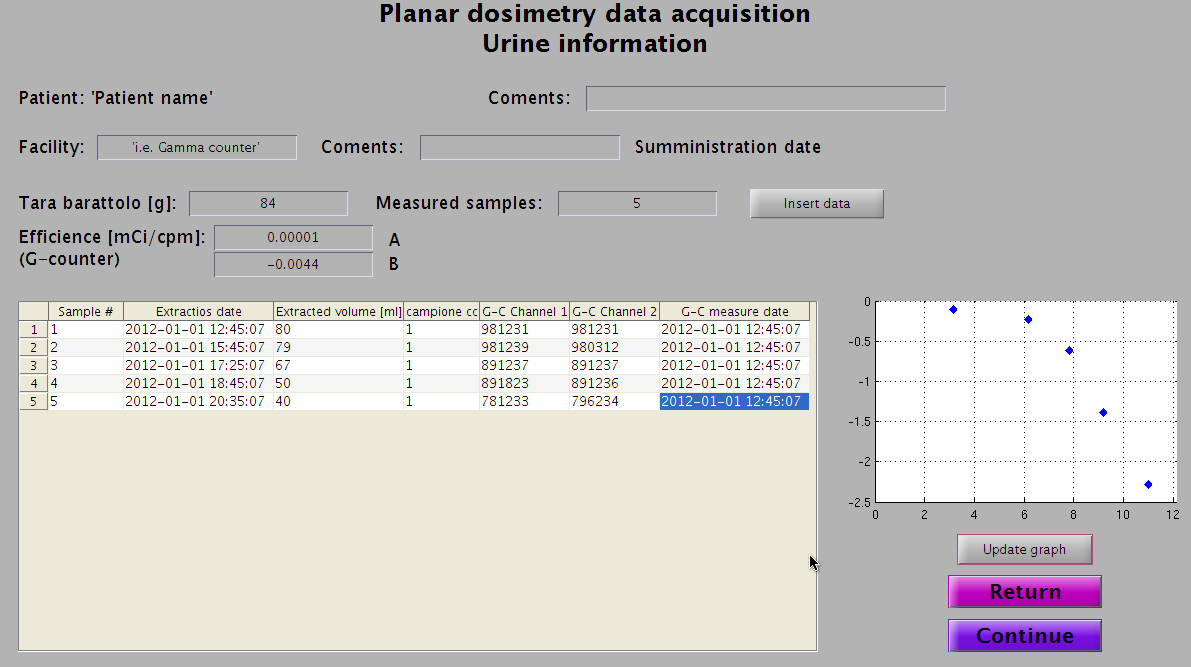
\includegraphics{imgs/planar-curves.png}

\end{frame}

\begin{frame}{3D dosimetry chartflow}
\protect\hypertarget{d-dosimetry-chartflow}{}

\includegraphics{imgs/3d-chartflow.png}

\end{frame}

\begin{frame}{3D dosimetry: \emph{GUI}}
\protect\hypertarget{d-dosimetry-gui}{}

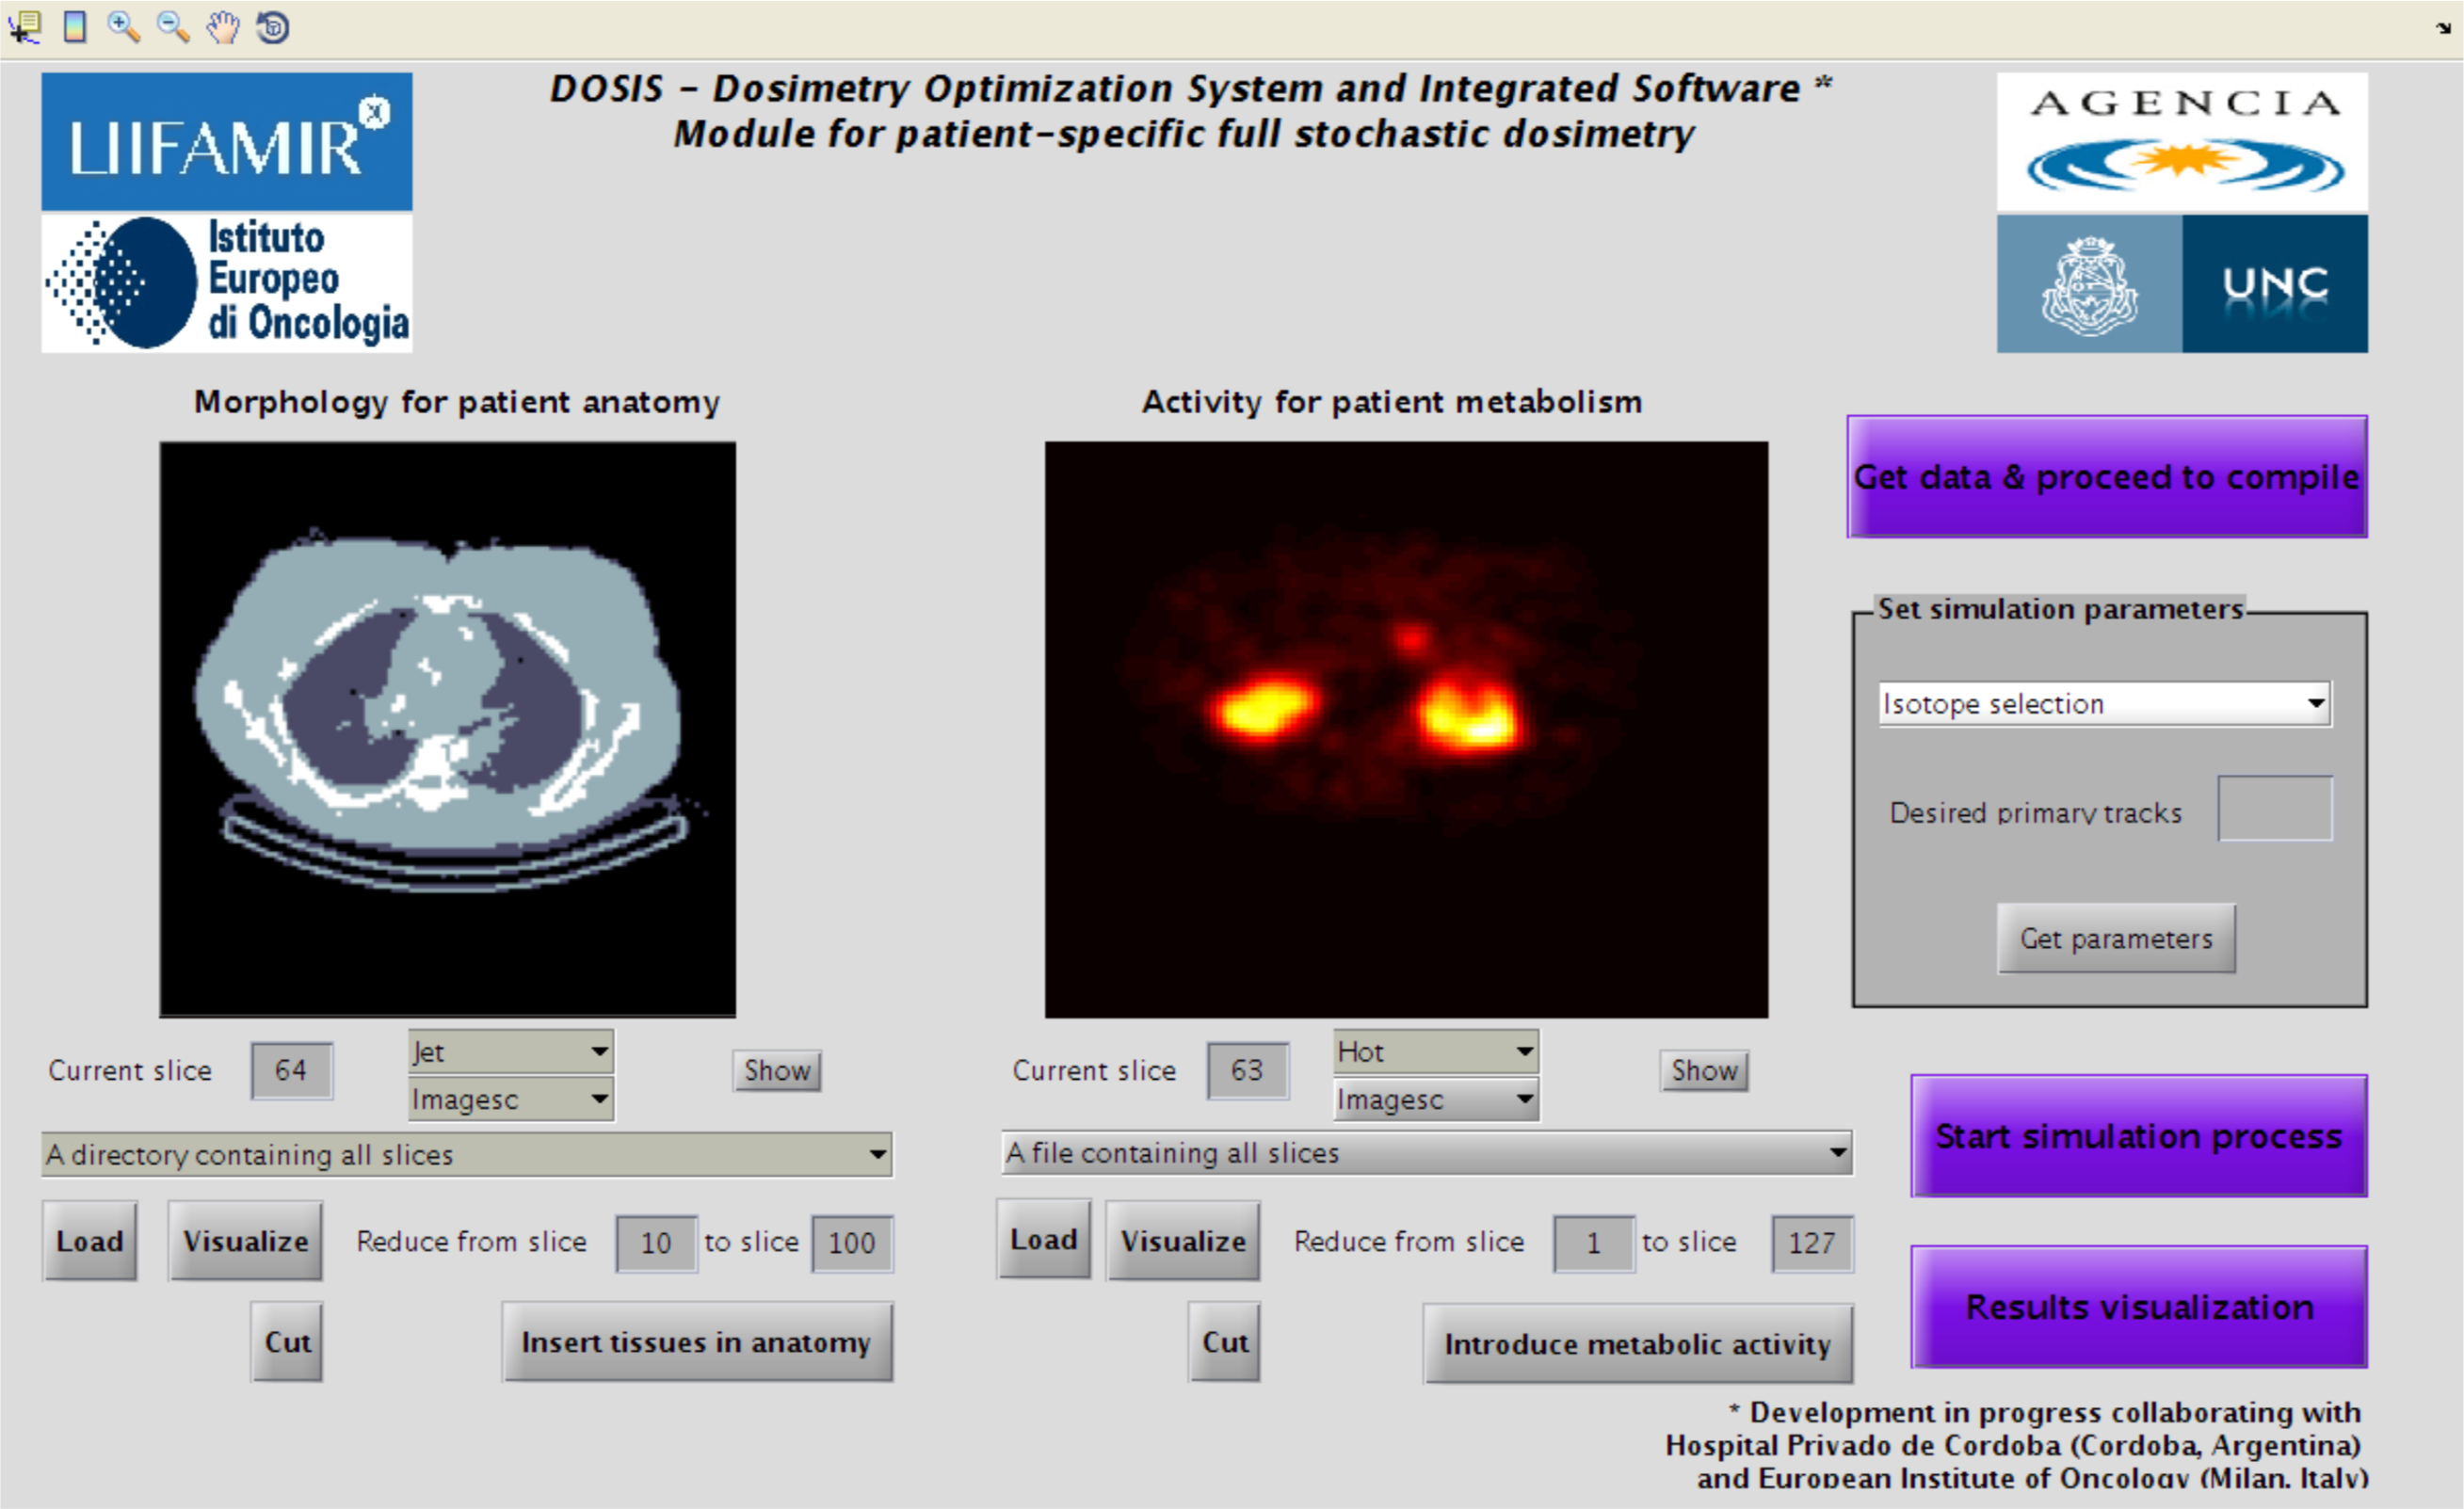
\includegraphics{imgs/3d-main.png}

\end{frame}

\begin{frame}{3D dosimetry: \emph{segmentation}}
\protect\hypertarget{d-dosimetry-segmentation}{}

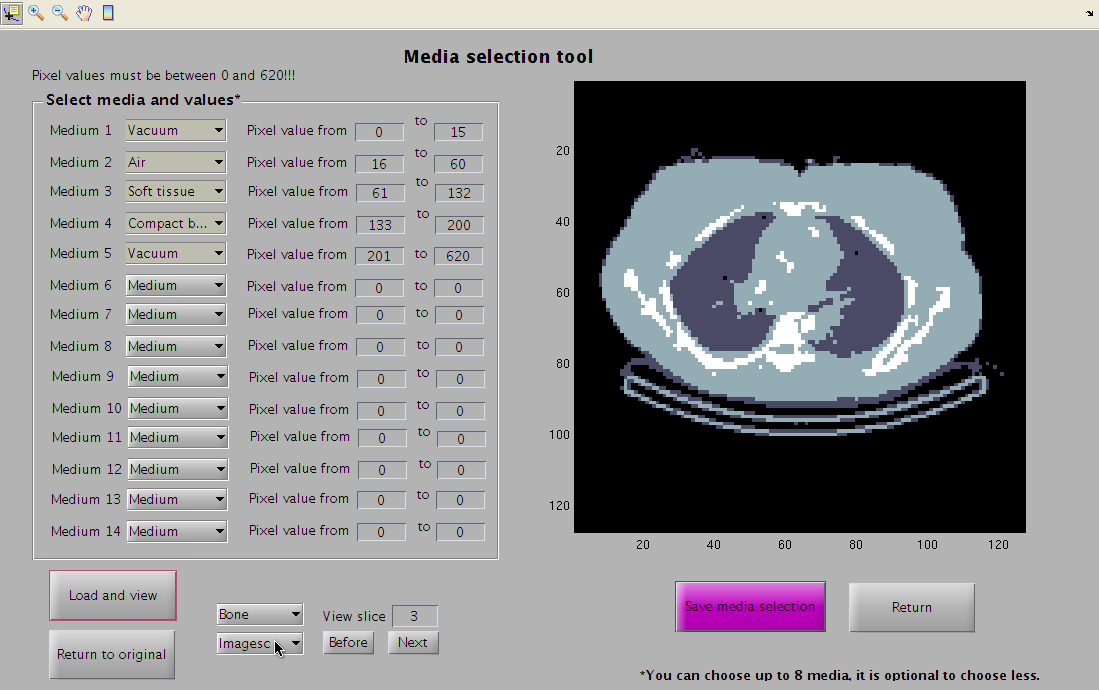
\includegraphics{imgs/3d-segmentation.png}

\end{frame}

\begin{frame}{3D dosimetry: \emph{visualization}}
\protect\hypertarget{d-dosimetry-visualization}{}

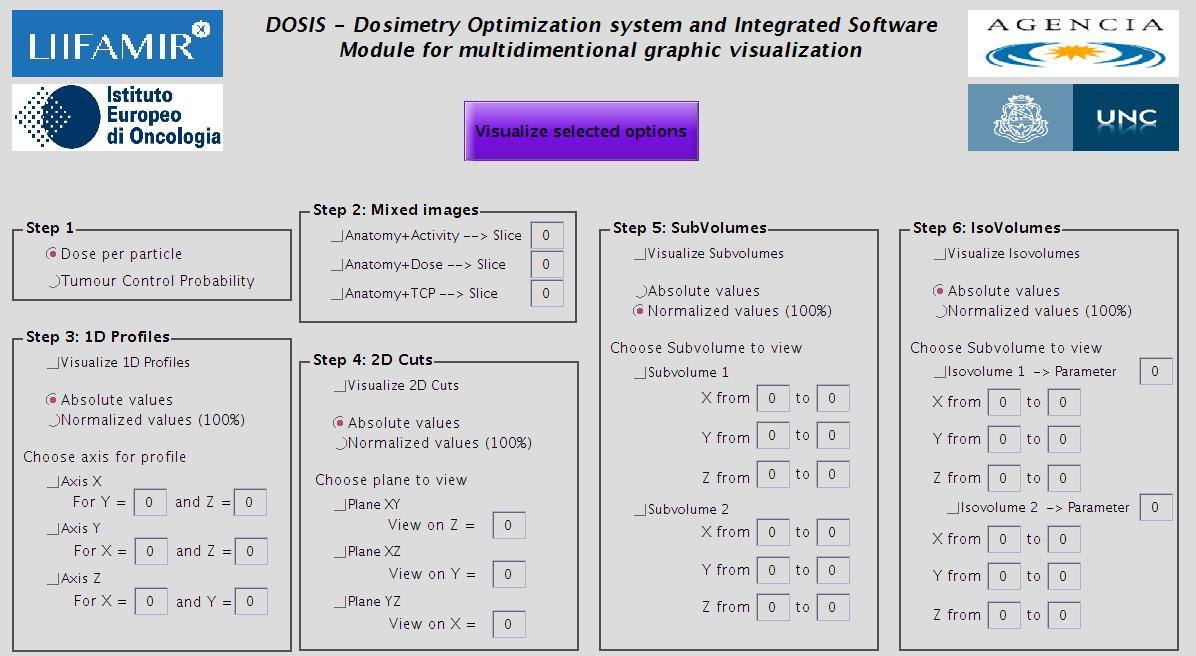
\includegraphics{imgs/3d-viz.jpg}

\end{frame}

\hypertarget{results}{%
\section{Results}\label{results}}

\begin{frame}{Monte Carlo simulations}
\protect\hypertarget{monte-carlo-simulations}{}

Comparison against bibliography on mathematical phantom

\begin{columns}
\begin{column}{.3\textwidth}
\begin{center}
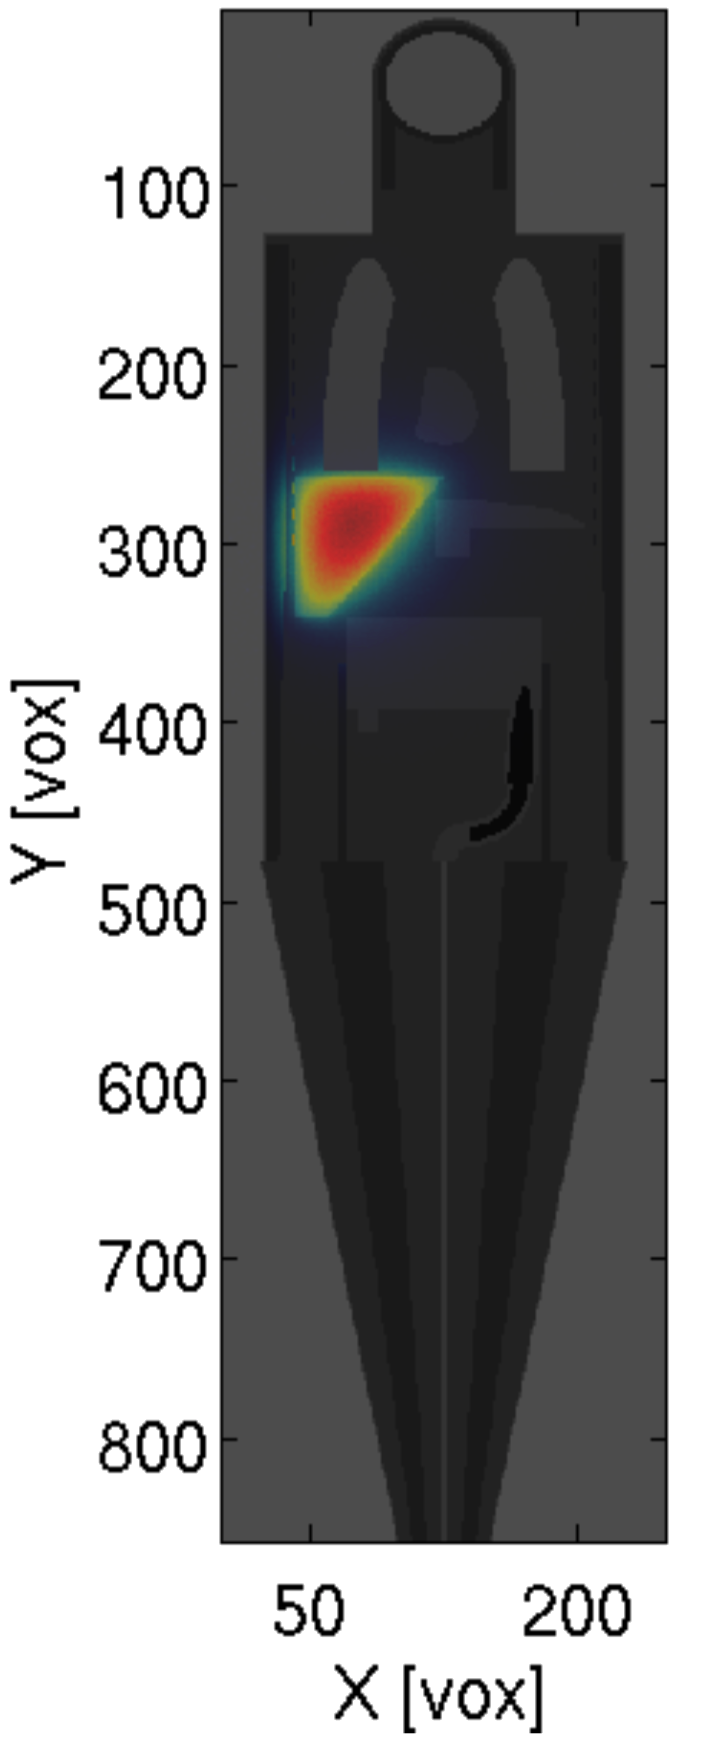
\includegraphics[height=.8\textheight]{imgs/mc_comparison.png}
\end{center}
\end{column}
\begin{column}{.7\textwidth}
\begin{center}
\begin{tabular}{l c c}
\hline
Organ & Reference\footnote{Cherry, Sorenson \& Phelps.{\it Physics in Nuclear Medicine.}} & DOSIS \\
\hline
Liver & 1 & 1 \\
Adrenals & 0.13 & 0.47 \\
Brain & 0.00025 & 0.00083 \\
Stomach & 0.46 & 0.82 \\
Kidneys & 0.09 & 0.32 \\
Lungs & 0.064 & 0.082 \\
Pancreas & 0.12 & 0.41 \\
Spleen & 0.022 & 0.042
\end{tabular}
\end{center}
\end{column}
\end{columns}

\end{frame}

\begin{frame}{MC results on patient images}
\protect\hypertarget{mc-results-on-patient-images}{}

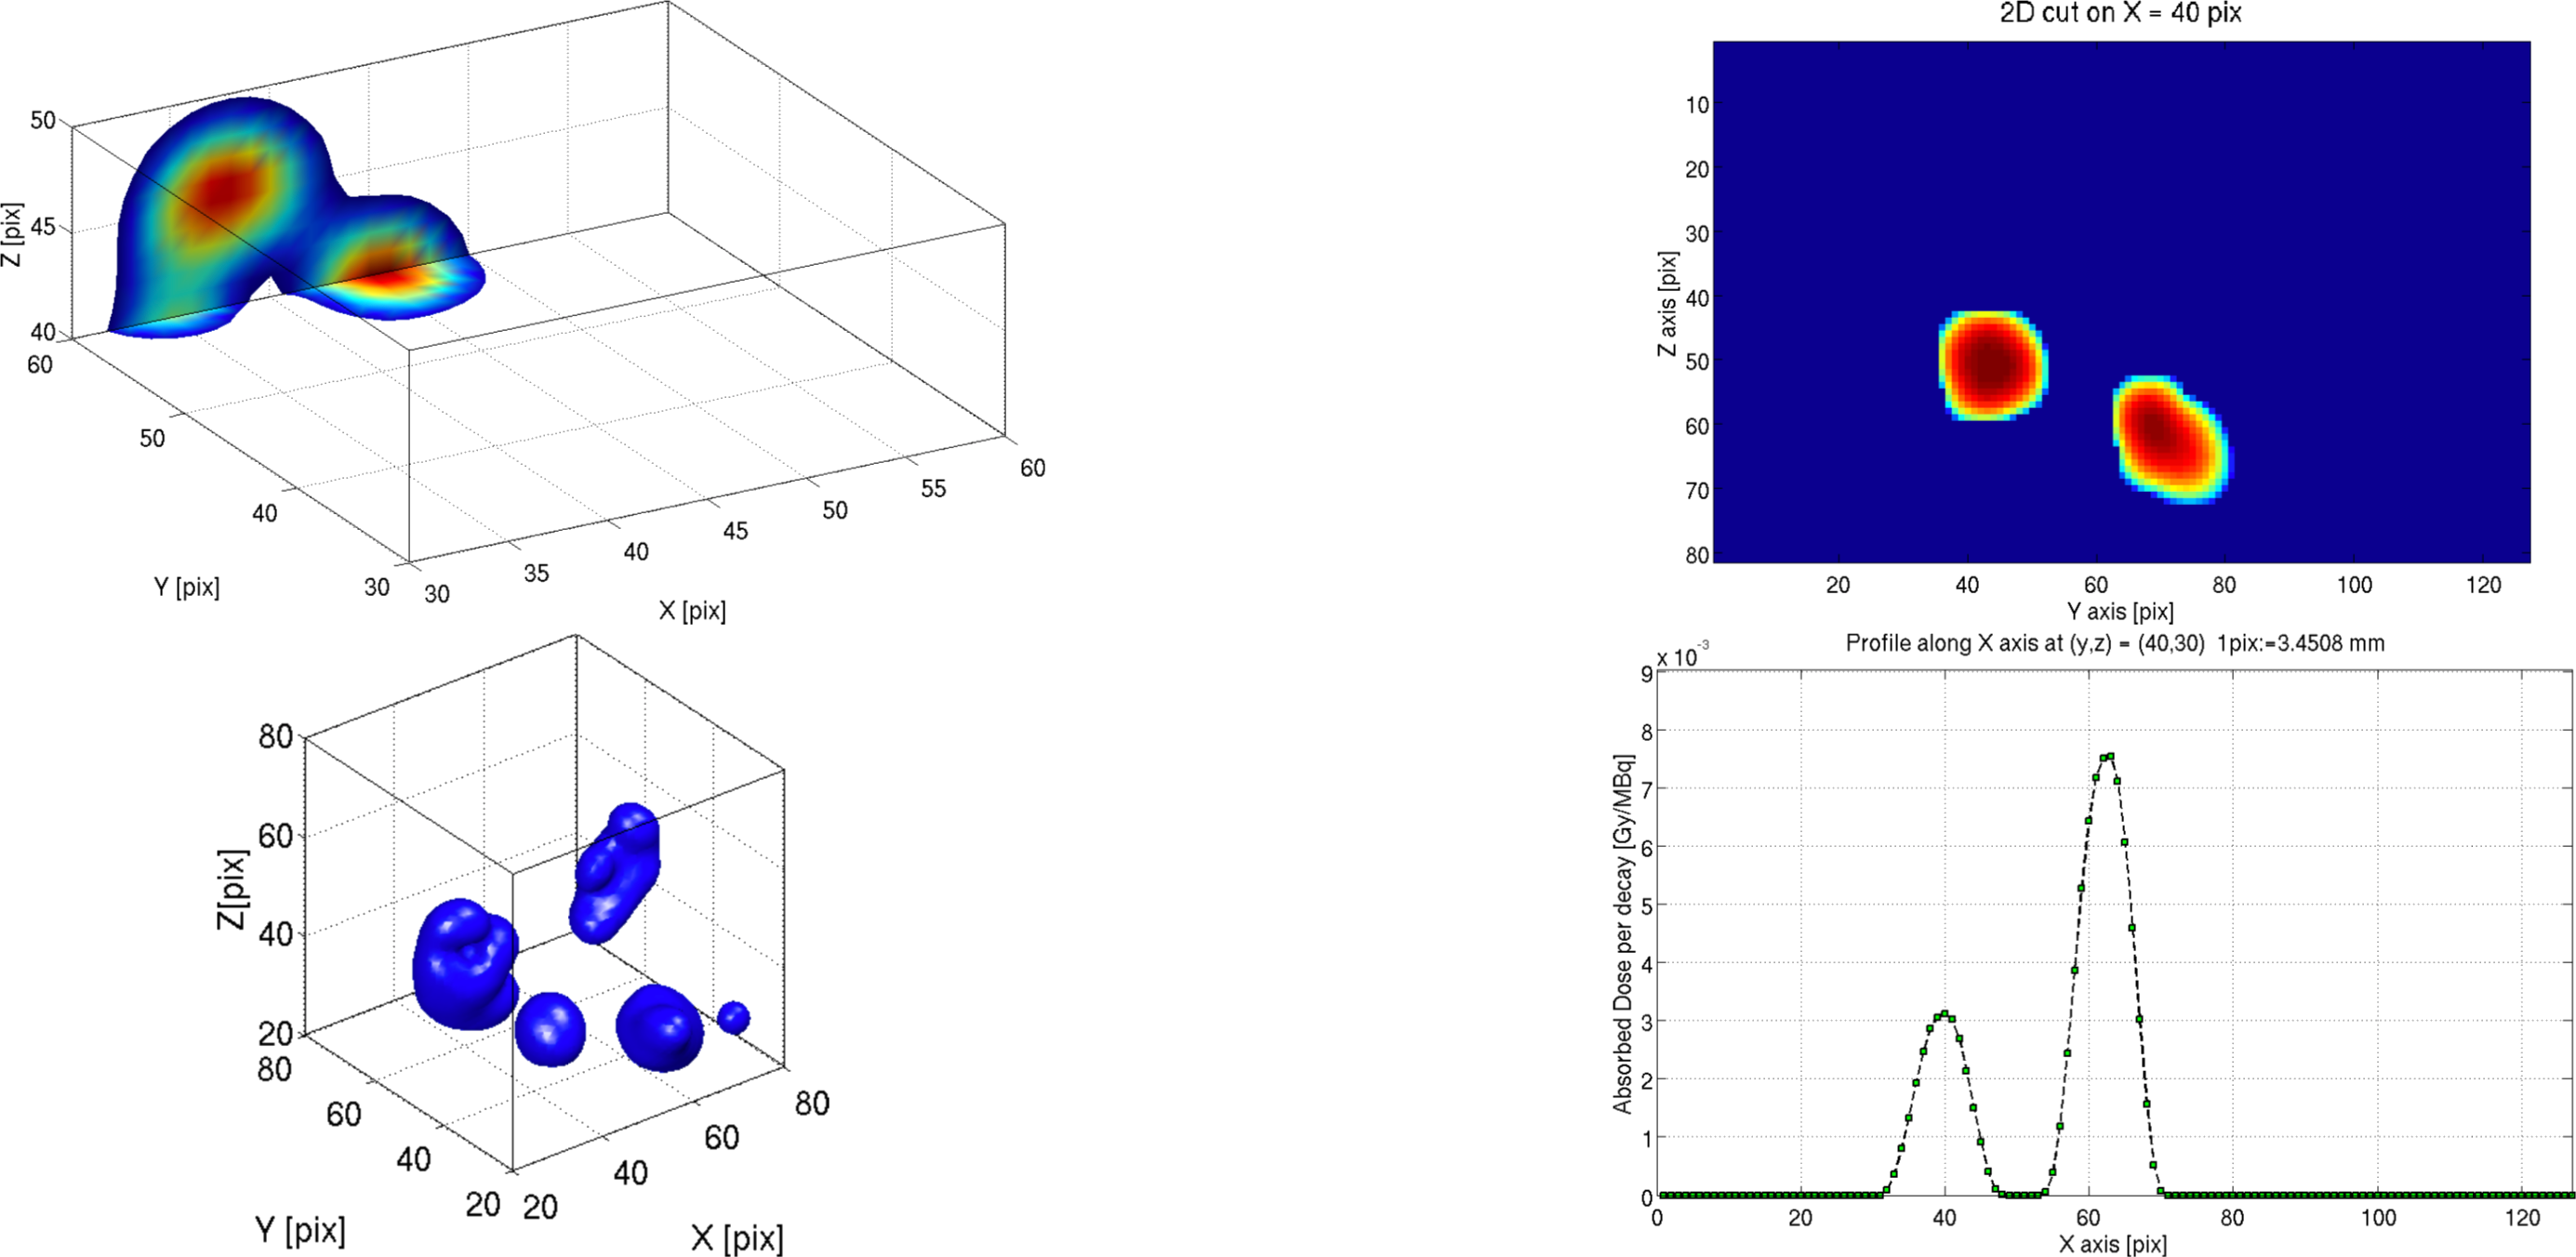
\includegraphics{imgs/mc_results.png}

\end{frame}

\begin{frame}{DOSIS results}
\protect\hypertarget{dosis-results}{}

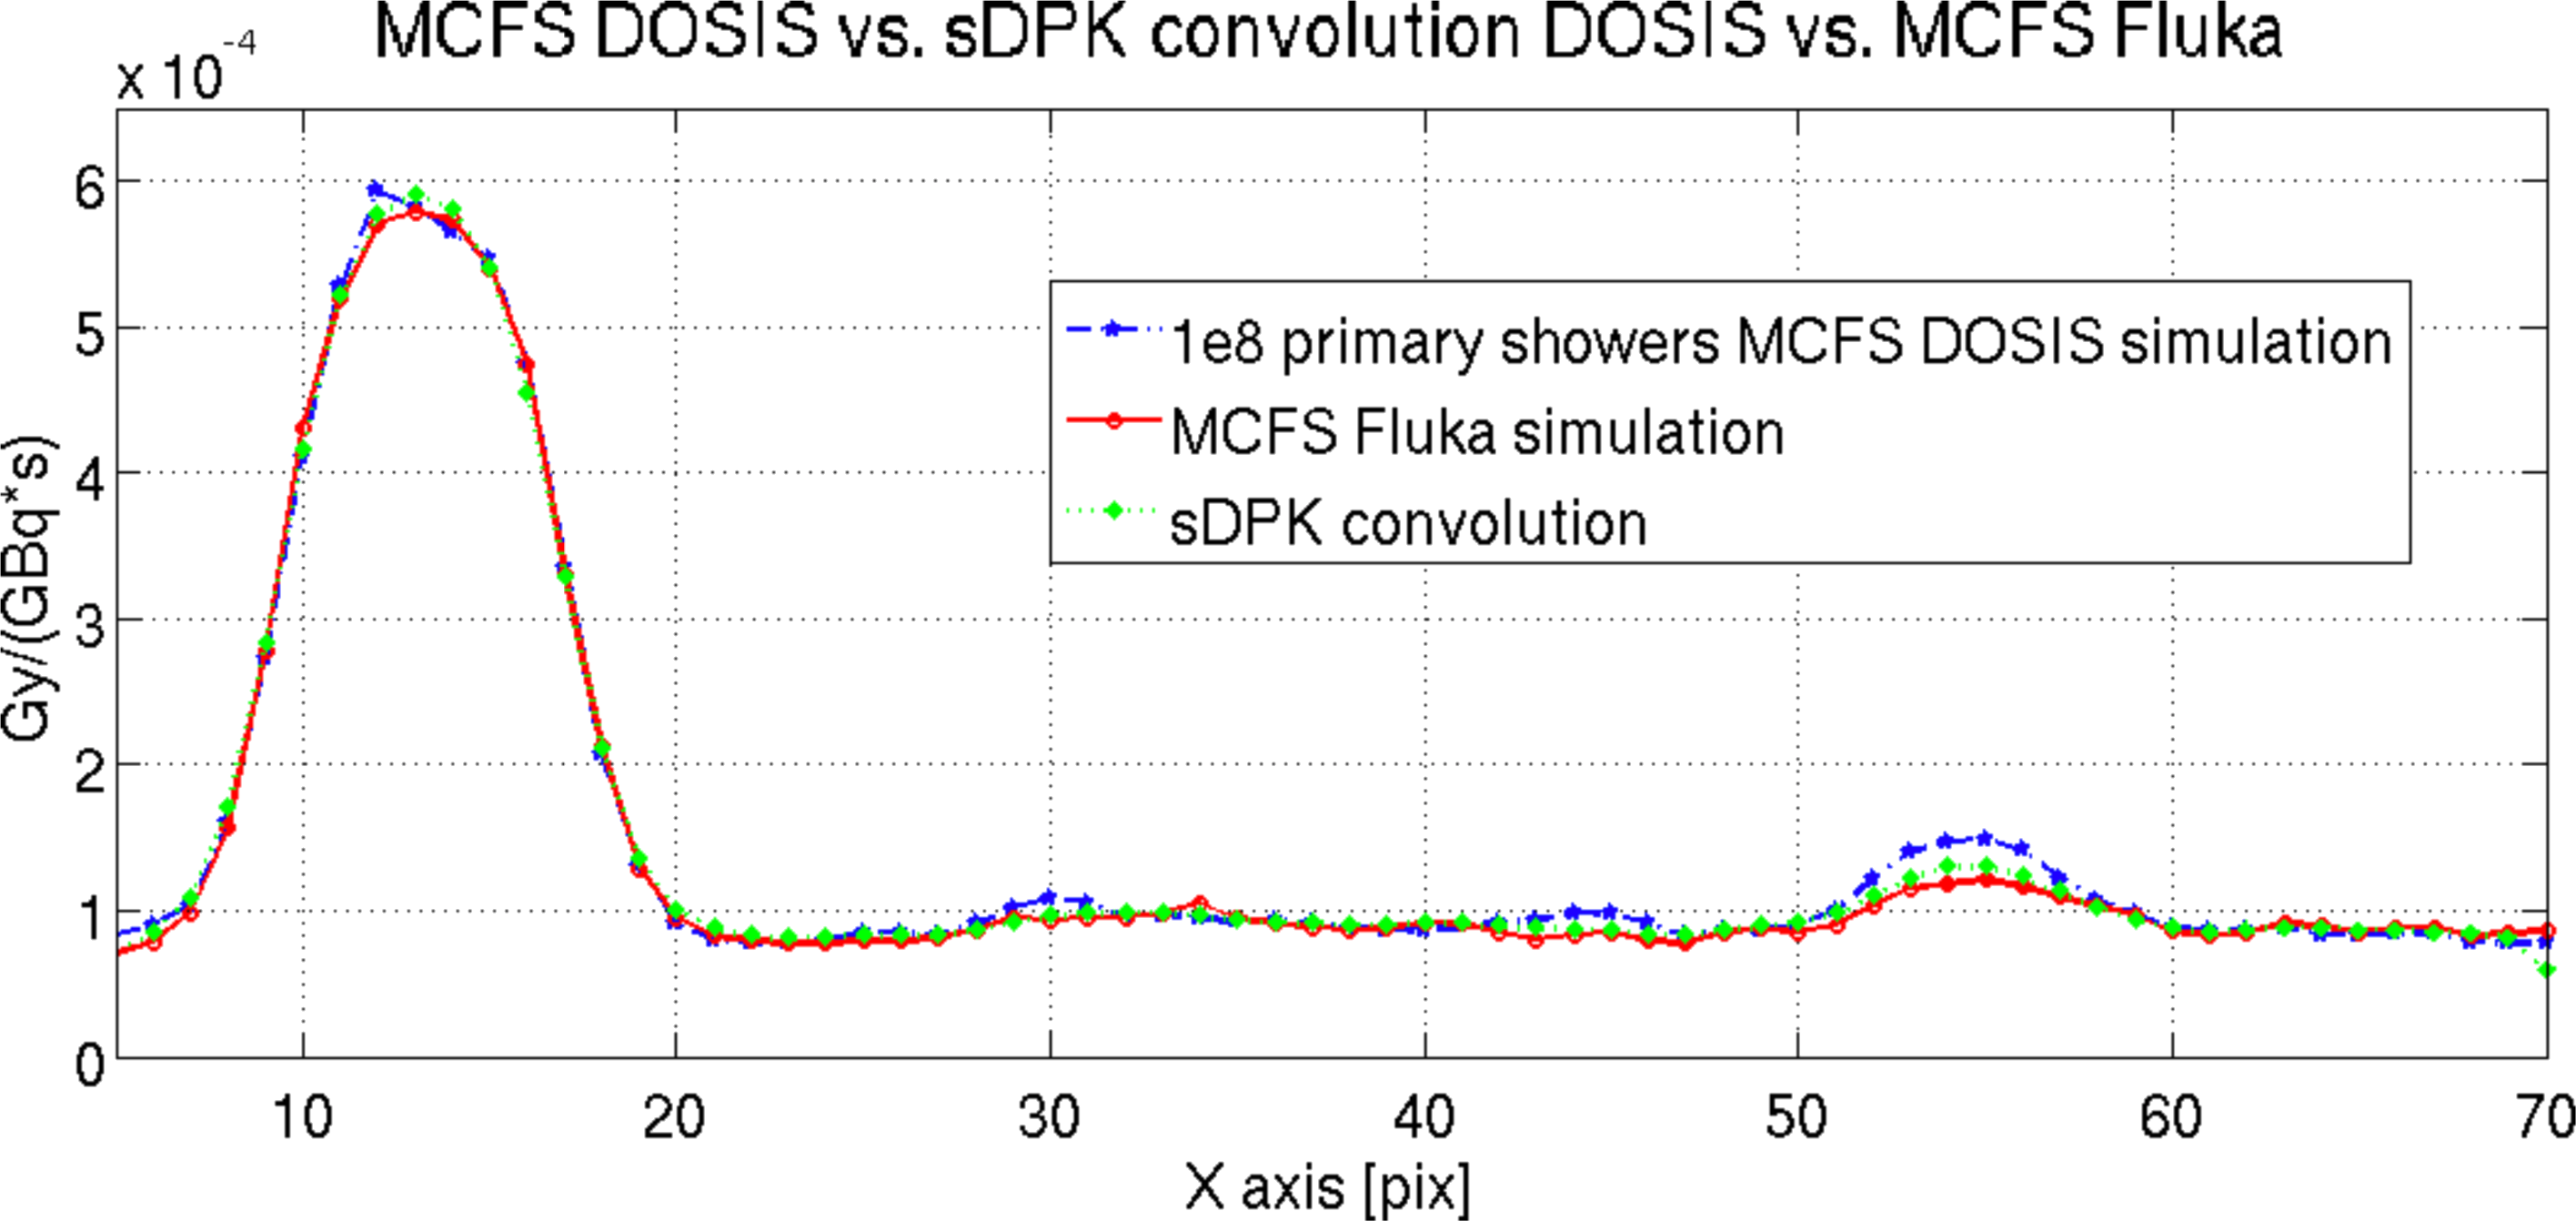
\includegraphics{imgs/dosis_results.png}

\end{frame}

\hypertarget{final-considerations}{%
\section{Final considerations}\label{final-considerations}}

\begin{frame}{DOSIS today}
\protect\hypertarget{dosis-today}{}

\begin{itemize}
\item
  The developed tool is capable of perfoming planar dosimetry
\item
  DOSIS the assessment of patient-specific 3D dosimetry at voxel level
  by means of MC simulations and DPK convolution
\item
  The tool is now in testing process for different situations with
  colleagues from IEO (Milán) and University of Lund (Sweeden)

  \begin{itemize}
  \tightlist
  \item
    analyzing effects of DPK convolutions when changing voxel size and
    activity distribution
  \item
    both DPK and MC calculations are being performed by DOSIS
  \item
    results are expected to be sent for publication end of the year
  \end{itemize}
\end{itemize}

\end{frame}

\begin{frame}{Uses: DPK}
\protect\hypertarget{uses-dpk}{}

\begin{center}
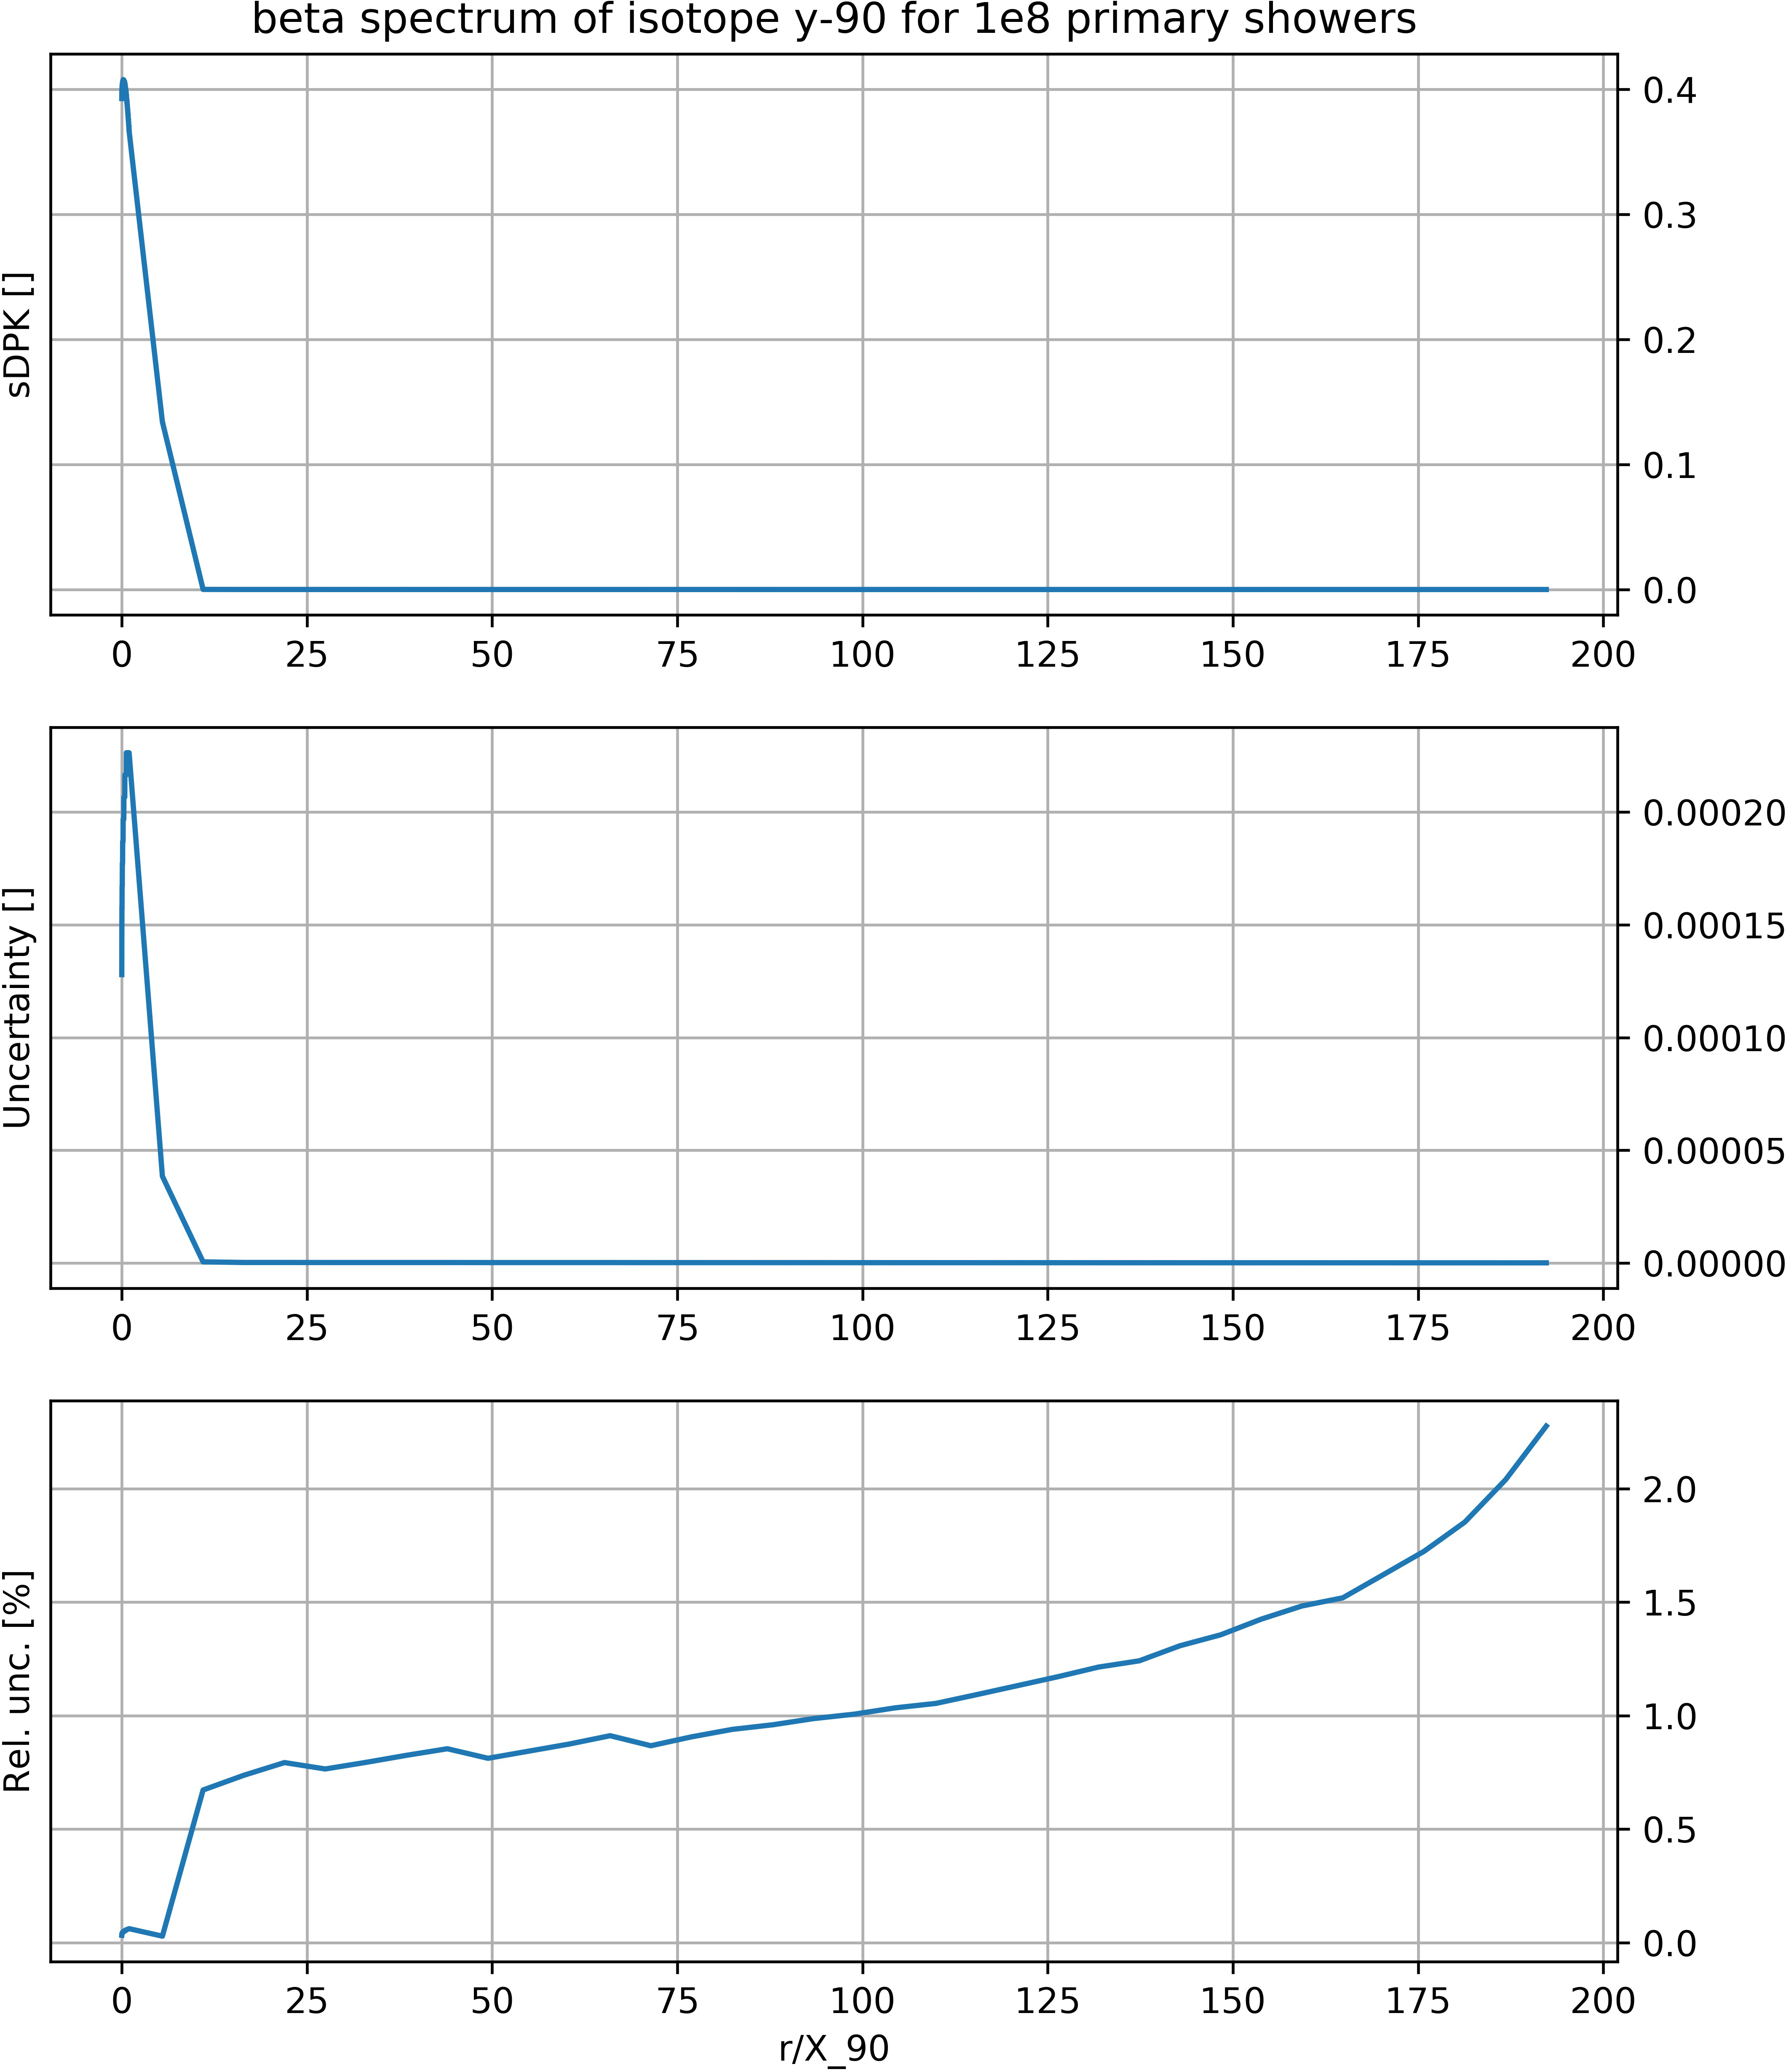
\includegraphics[width=.33\textwidth]{imgs/now1.jpg}
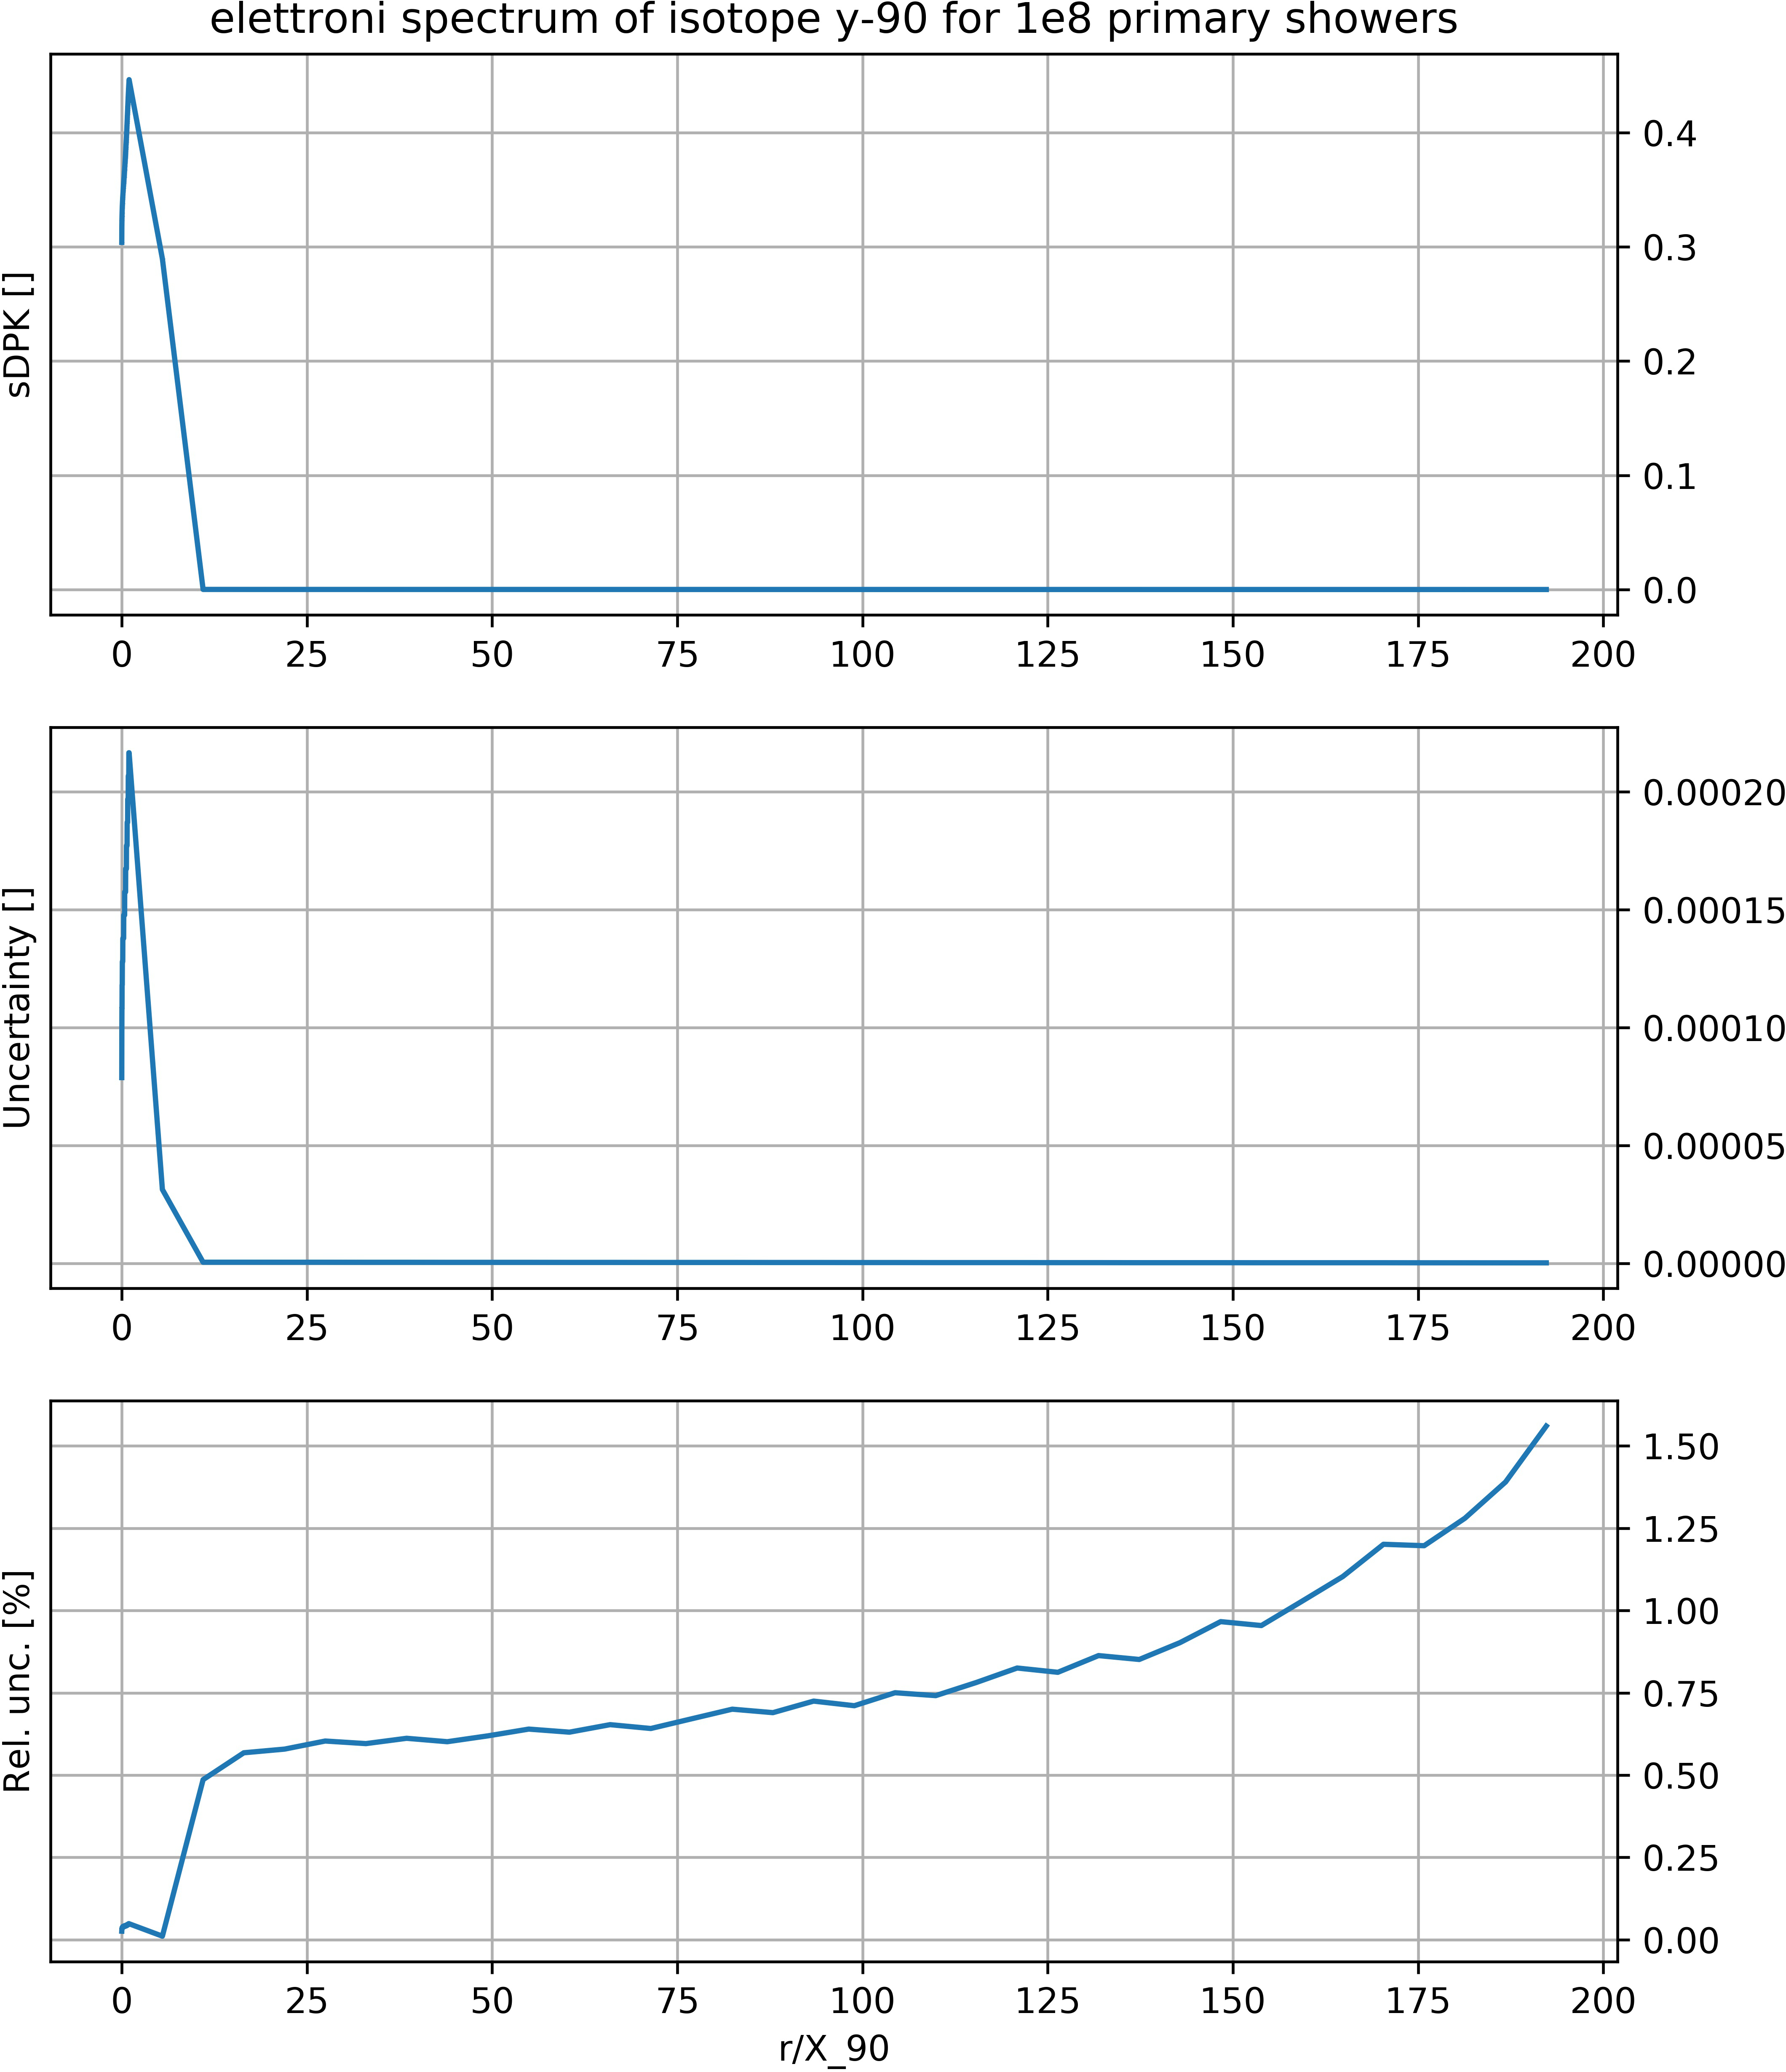
\includegraphics[width=.33\textwidth]{imgs/now2.jpg}
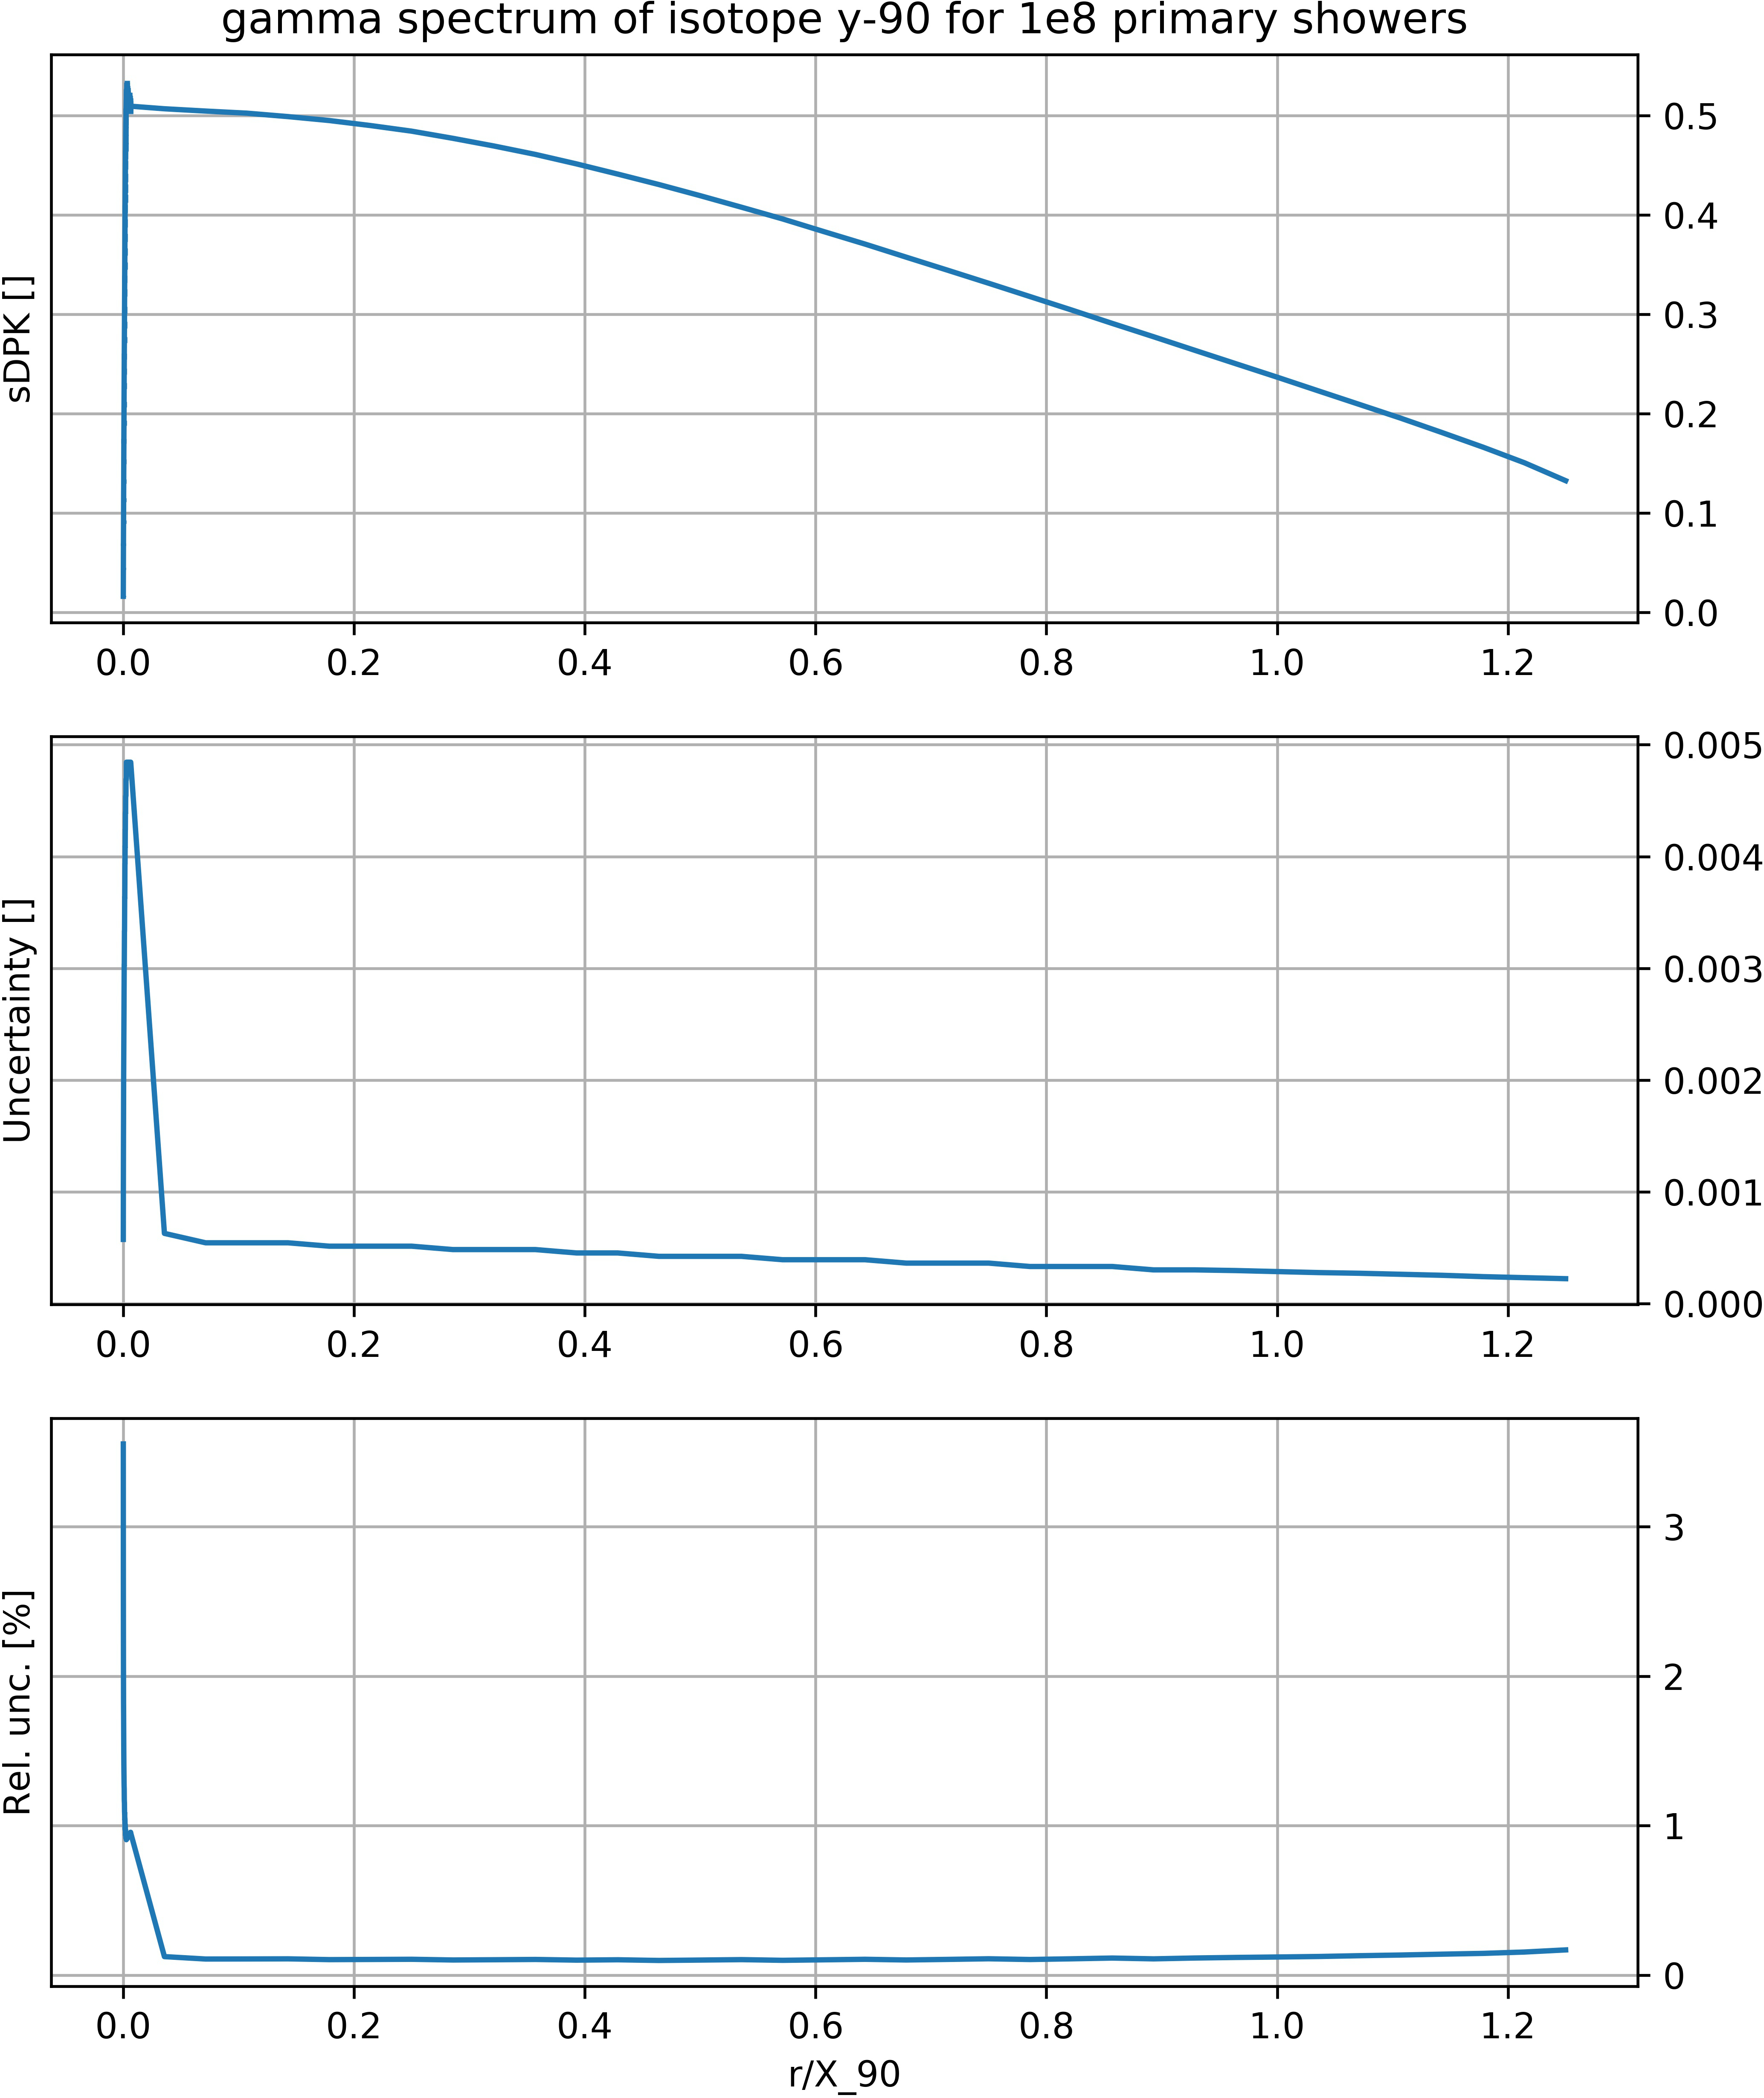
\includegraphics[width=.33\textwidth]{imgs/now3.jpg}
\end{center}

\end{frame}

\begin{frame}{Uses: MC}
\protect\hypertarget{uses-mc}{}

\begin{center}
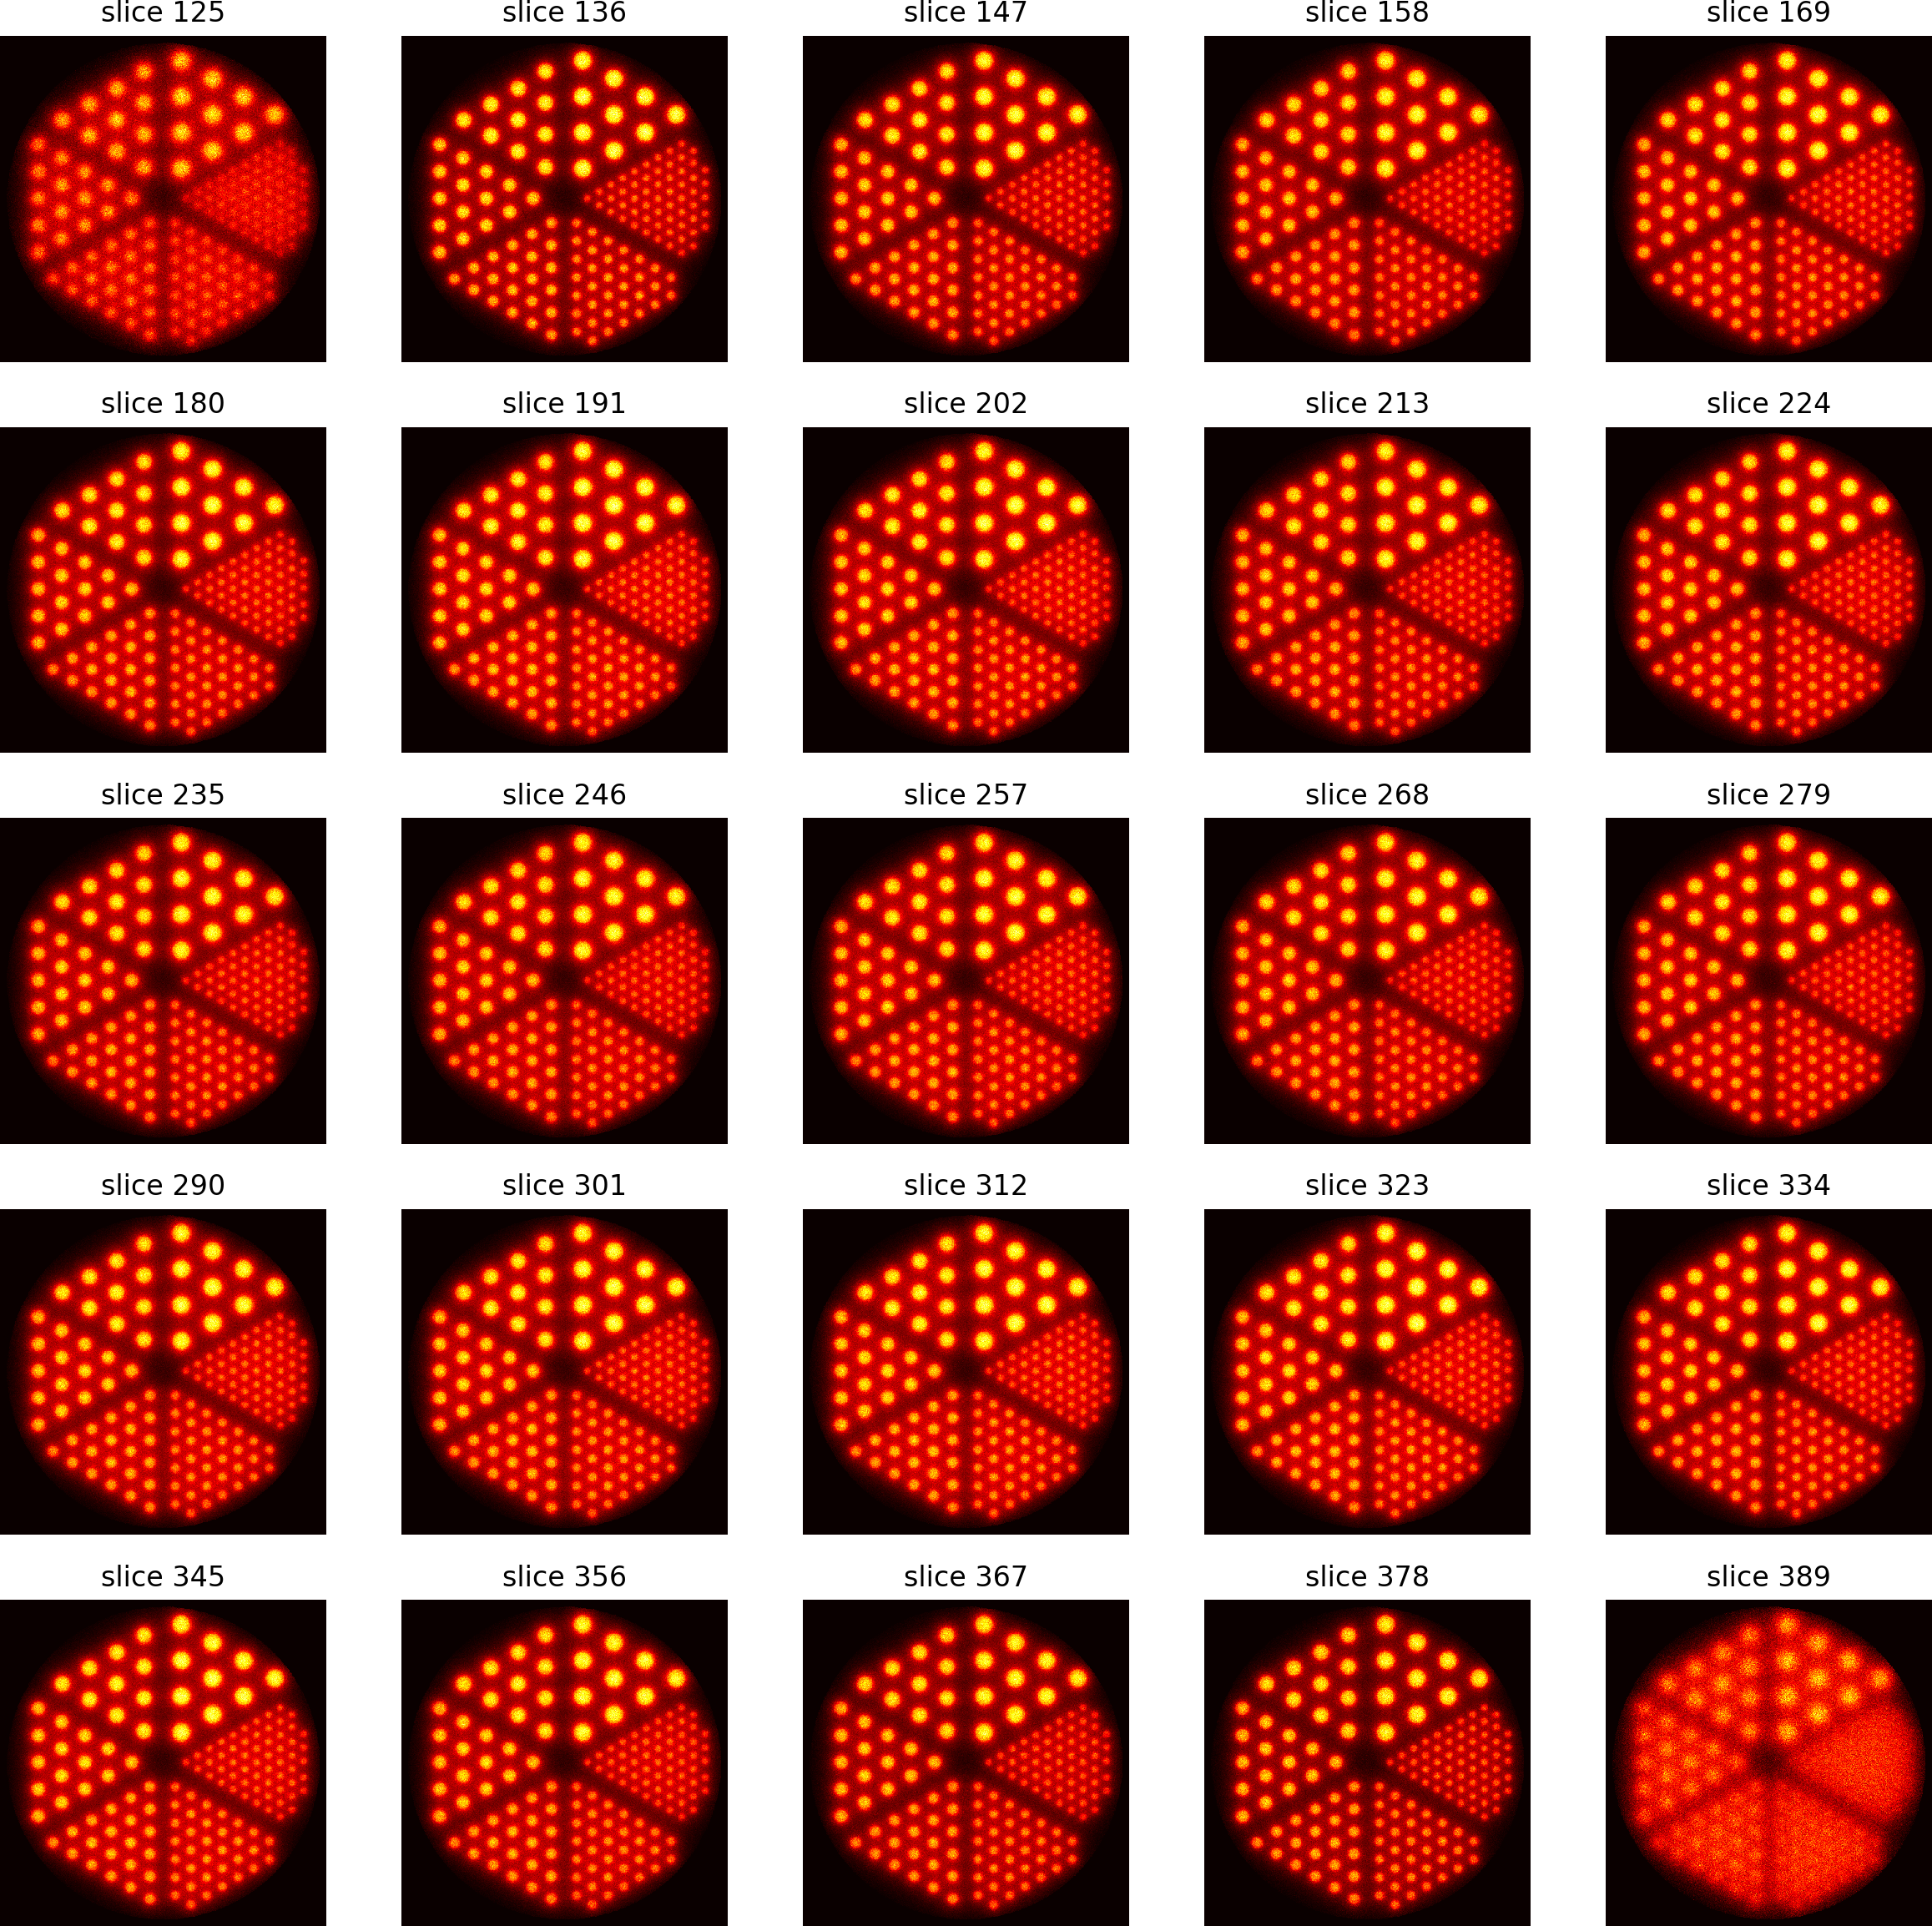
\includegraphics[width=.75\textheight]{imgs/now4.png}
\end{center}

\end{frame}

\begin{frame}{Next Work}
\protect\hypertarget{next-work}{}

\begin{itemize}
\item
  move to free languages like Python
\item
  improve GUI and segmentation modules
\item
  develope FLUKA implementation in order to add alpha emitters
\item
  test the DOSIS with measurements and other calculation softwares
\end{itemize}

\end{frame}

\hypertarget{thanks}{%
\section{Thanks!}\label{thanks}}

\begin{frame}{Visit us in Córdoba!}
\protect\hypertarget{visit-us-in-cordoba}{}

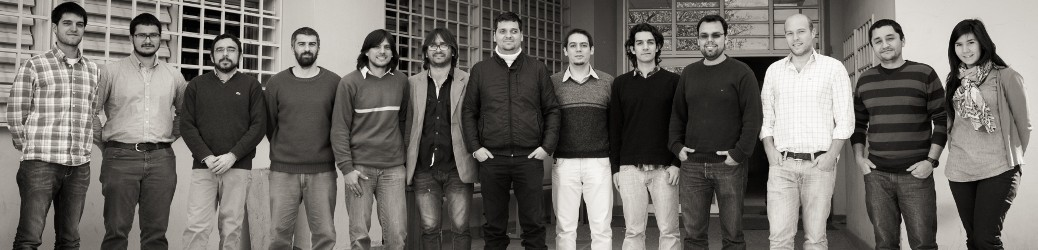
\includegraphics{imgs/liifamir.jpg}

\begin{center}
www.liifamirx.famaf.unc.edu.ar\\
\vspace{.4cm}
\footnotesize download this presentation from: github.com/pap84/oral-jfmf2018
\end{center}

\end{frame}

\end{document}
